% ==================================================================
%  §8.2  微分
%  源：徐森林、薛春华《数学分析》第二册，印刷页 70-95 (PDF p. 76-101)
%  底本：PaddleOCR-VL-1.6 JSON/MD 识别结果，人工逐字核校与公式精修
%  规范：全西文标点，忠实原文定义、注、定理、例题、练习题编号与推导
% ==================================================================

\section{微分}\label{sec:8.2}

在 8.1 节已经介绍了方向导数与偏导数两个重要概念, 这一节将介绍另一个重要概念, 就是微分.

\begin{definition}\label{def:8.2.1}
设 $U \subset \mathbb{R}^{n}$ 为开集, $f: U \to \mathbb{R}^{1}$ 为 $n$ 元函数,
\[
  \boldsymbol{x}^{0} = \begin{pmatrix} x_{1}^{0} \\ \vdots \\ x_{n}^{0} \end{pmatrix} \in U, \quad
  \boldsymbol{x} = \begin{pmatrix} x_{1} \\ \vdots \\ x_{n} \end{pmatrix} \in U, \quad
  \Delta\boldsymbol{x} = \begin{pmatrix} \Delta x_{1} \\ \vdots \\ \Delta x_{n} \end{pmatrix}
  = \begin{pmatrix} x_{1} - x_{1}^{0} \\ \vdots \\ x_{n} - x_{n}^{0} \end{pmatrix}
  = \boldsymbol{x} - \boldsymbol{x}^{0} \in \mathbb{R}^{n},
\]
$\boldsymbol{A} = (a_{1}, a_{2}, \cdots, a_{n})$ 为行向量, $a_{i} \in \mathbb{R}$ 为常数 (与 $\Delta\boldsymbol{x}$ 无关).

如果
\begin{align*}
  \Delta f &= f(\boldsymbol{x}^{0} + \Delta\boldsymbol{x}) - f(\boldsymbol{x}^{0}) = \boldsymbol{A}\Delta\boldsymbol{x} + o(\|\Delta\boldsymbol{x}\|), \quad \|\Delta\boldsymbol{x}\| \to 0, \\
  f(x_{1}^{0} + \Delta x_{1}, x_{2}^{0} + \Delta x_{2}, \cdots, x_{n}^{0} + \Delta x_{n}) &- f(x_{1}^{0}, x_{2}^{0}, \cdots, x_{n}^{0}) \\
  &\quad = a_{1}\Delta x_{1} + a_{2}\Delta x_{2} + \cdots + a_{n}\Delta x_{n} + o\Big(\sqrt{\sum_{i=1}^{n}(\Delta x_{i})^{2}}\Big),
\end{align*}
即
\begin{align*}
  \Delta f &= f(\boldsymbol{x}) - f(\boldsymbol{x}^{0}) = \boldsymbol{A}(\boldsymbol{x} - \boldsymbol{x}^{0}) + o(\|\boldsymbol{x} - \boldsymbol{x}^{0}\|), \quad \|\boldsymbol{x} - \boldsymbol{x}^{0}\| \to 0, \\
  f(x_{1}, x_{2}, \cdots, x_{n}) &- f(x_{1}^{0}, x_{2}^{0}, \cdots, x_{n}^{0}) \\
  &\quad = a_{1}(x_{1} - x_{1}^{0}) + a_{2}(x_{2} - x_{2}^{0}) + \cdots + a_{n}(x_{n} - x_{n}^{0}) + o\Big(\sqrt{\sum_{i=1}^{n}(x_{i} - x_{i}^{0})^{2}}\Big),
\end{align*}
则称 $f$ 在 $\boldsymbol{x}^{0}$ 点处\textbf{可微}. 记
\begin{align*}
  &\mathrm{d}f(\boldsymbol{x}^{0}): \mathbb{R}^{n} \to \mathbb{R}^{1}, \\
  &\mathrm{d}f(\boldsymbol{x}^{0})(\Delta\boldsymbol{x}) = \boldsymbol{A}\Delta\boldsymbol{x}, \quad \Delta\boldsymbol{x} \in \mathbb{R}^{n}.
\end{align*}
显然, $\mathrm{d}f(\boldsymbol{x}^{0})$ 为线性映射, 称 $\mathrm{d}f(\boldsymbol{x}^{0})$ 为 $f$ 在点 $\boldsymbol{x}^{0} \in U$ 处的\textbf{微分}.
\end{definition}

\begin{theorem}\label{thm:8.2.1}
$f$ 在 $\boldsymbol{x}^{0}$ 处可微, 必有 $f$ 在 $\boldsymbol{x}^{0}$ 处连续. 但反之不真.
\end{theorem}

\begin{proof}
因为 $f$ 在 $\boldsymbol{x}^{0}$ 处可微, 所以
\[
  \lim_{\boldsymbol{x} \to \boldsymbol{x}^{0}}f(\boldsymbol{x}) = \lim_{\boldsymbol{x} \to \boldsymbol{x}^{0}}[f(\boldsymbol{x}^{0}) + \boldsymbol{A}(\boldsymbol{x} - \boldsymbol{x}^{0}) + o(\|\boldsymbol{x} - \boldsymbol{x}^{0}\|)] = f(\boldsymbol{x}^{0}) + \boldsymbol{A}\boldsymbol{0} + 0 = f(\boldsymbol{x}^{0}),
\]
即 $f$ 在 $\boldsymbol{x}^{0}$ 点处连续.

但反之不真. 例如, 一元函数 $f(x) = |x|$ 在 $x^{0} = 0$ 点处连续, 而
\[
  |x| - |0| = A(x - 0) + o(|x - 0|).
\]
无论 $A$ 为何实数上式总不成立. 因此, $f(x) = |x|$ 在 $x^{0} = 0$ 点处不可微.
\end{proof}

\begin{theorem}\label{thm:8.2.2}
一元函数 $f$ 在 $x^{0}$ 点可微 $\Leftrightarrow$ $f$ 在 $x^{0}$ 点可导. 并且, $A = f'(x^{0})$ (\cref{fig:8.2.1}).
\end{theorem}

\begin{figure}[htbp]
  \centering
  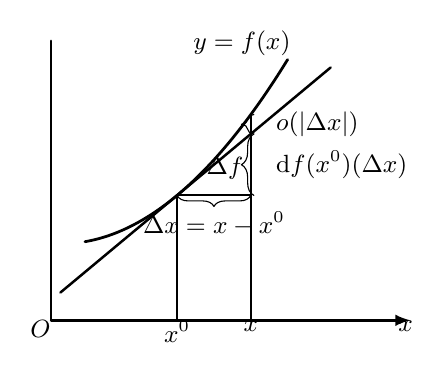
\begin{tikzpicture}[x=0.78cm, y=0.78cm, >=latex, line cap=round, line join=round]
    % ---------- 坐标架 ----------
    \draw[line width=0.9pt] (0, 0) -- (0, 4.55);
    \draw[line width=0.9pt, ->] (0, 0) -- (5.85, 0);
    \node[below left=-1pt, inner sep=1pt] at (0, 0) {\small $O$};
    \node[below left=-1pt, inner sep=1pt] at (5.90, 0) {\small $x$};
    % ---------- 曲线 y = f(x) ----------
    \draw[line width=1.0pt, domain=0.55:3.85, samples=80]
      plot (\x, {1.28 + 0.1727*(\x-0.55) + 0.22*(\x-0.55)*(\x-0.55)});
    \node[anchor=south east, inner sep=1pt] at (3.95, 4.26) {\small $y = f(x)$};
    % ---------- 切线（过 P_0 = (x^0, f(x^0))） ----------
    \draw[line width=0.9pt] (0.15, 0.452) -- (4.55, 4.116);
    % ---------- 竖直/水平辅助线 ----------
    \draw[line width=0.8pt] (2.05, 0) -- (2.05, 2.034);
    \draw[line width=0.8pt] (3.25, 0) -- (3.25, 3.350);
    \draw[line width=0.8pt] (2.05, 2.034) -- (3.25, 2.034);
    \node[below=-1pt, inner sep=1pt] at (2.05, 0) {\small $x^{0}$};
    \node[below=-1pt, inner sep=1pt] at (3.25, 0) {\small $x$};
    % ---------- 大括号与注记 ----------
    \draw[decorate, decoration={brace, amplitude=4pt, mirror}] (2.05, 2.034) -- (3.25, 2.034);
    \node[below=4pt, inner sep=1pt] at (2.65, 2.00) {\small $\Delta x = x - x^{0}$};
    \draw[decorate, decoration={brace, amplitude=4.5pt}] (3.30, 2.034) -- (3.30, 3.033);
    \draw[decorate, decoration={brace, amplitude=4.5pt}] (3.30, 3.033) -- (3.30, 3.350);
    \node[right=6pt, inner sep=1pt] at (3.34, 2.53) {\small $\mathrm{d}f(x^{0})(\Delta x)$};
    \node[right=6pt, inner sep=1pt] at (3.34, 3.19) {\small $o(|\Delta x|)$};
    \node[anchor=east, inner sep=1pt] at (3.18, 2.47) {\small $\Delta f$};
  \end{tikzpicture}
  \caption{}\label{fig:8.2.1}
\end{figure}

\begin{proof}
($\Rightarrow$) 因为 $f$ 在 $x^{0}$ 点可微, 即
\[
  f(x) - f(x^{0}) = A(x - x^{0}) + o(|x - x^{0}|) = A(x - x^{0}) + o(x - x^{0}),
\]
则
\begin{align*}
  \lim_{x \to x^{0}}\frac{f(x) - f(x^{0})}{x - x^{0}}
  &= \lim_{x \to x^{0}}\Big[A + \frac{o(|x - x^{0}|)}{x - x^{0}}\Big] \\
  &= A + 0 = A,
\end{align*}
从而 $f$ 在 $x^{0}$ 点处可导, 且 $f'(x^{0}) = A$.

($\Leftarrow$) 因为 $f$ 在 $x^{0}$ 点可导, 所以
\begin{align*}
  \lim_{x \to x^{0}}\frac{f(x) - f(x^{0}) - f'(x^{0})(x - x^{0})}{x - x^{0}}
  &= \lim_{x \to x^{0}}\Big[\frac{f(x) - f(x^{0})}{x - x^{0}} - f'(x^{0})\Big] \\
  &= f'(x^{0}) - f'(x^{0}) = 0.
\end{align*}
由此得到
\[
  f(x) - f(x^{0}) - f'(x^{0})(x - x^{0}) = o(|x - x^{0}|),
\]
\[
  f(x) - f(x^{0}) = f'(x^{0})(x - x^{0}) + o(|x - x^{0}|).
\]
这就证明了 $f$ 在点 $x^{0}$ 处是可微的.
\end{proof}

\cref{thm:8.2.2}表明, 当 $n = 1$ 时, $f$ 在 $x^{0}$ 可微与可导是彼此等价的. 是否可以指望当 $n \geqslant 2$ 时, $f$ 在 $x^{0}$ 点可微与 $f$ 在 $x^{0}$ 点有偏导数是彼此等价的呢? 下面的定理给出了明确的回答.

\begin{theorem}[可微的必要条件]\label{thm:8.2.3}
$n$ 元函数 $f$ 在 $\boldsymbol{x}^{0}$ 点处可微, 则 $f$ 在 $\boldsymbol{x}^{0}$ 点处有一阶偏导数 $f_{x_{i}}'(\boldsymbol{x}^{0})$, $i = 1, 2, \cdots, n$, 且 $\boldsymbol{A} = \boldsymbol{J}\boldsymbol{f}(\boldsymbol{x}^{0}) = (f_{x_{1}}'(\boldsymbol{x}^{0}), f_{x_{2}}'(\boldsymbol{x}^{0}), \cdots, f_{x_{n}}'(\boldsymbol{x}^{0}))$. 但反之不真.
\end{theorem}

\begin{proof}
设 $n$ 元函数 $f$ 在 $\boldsymbol{x}^{0}$ 点处可微, 令
\[
  x_{j} - x_{j}^{0} = 0, \quad j = 1, 2, \cdots, i - 1, i + 1, \cdots, n,
\]
可以得到
\begin{align*}
  &f(x_{1}^{0}, x_{2}^{0}, \cdots, x_{i-1}^{0}, x_{i}, x_{i+1}^{0}, \cdots, x_{n}^{0}) - f(x_{1}^{0}, x_{2}^{0}, \cdots, x_{i-1}^{0}, x_{i}^{0}, x_{i+1}^{0}, \cdots, x_{n}^{0}) \\
  &= a_{i}(x_{i} - x_{i}^{0}) + o(|x_{i} - x_{i}^{0}|) = a_{i}(x_{i} - x_{i}^{0}) + o(x_{i} - x_{i}^{0}).
\end{align*}
于是,
\begin{align*}
  f_{x_{i}}'(\boldsymbol{x}^{0})
  &= \lim_{x_{i} \to x_{i}^{0}}\frac{f(x_{1}^{0}, x_{2}^{0}, \cdots, x_{i-1}^{0}, x_{i}, x_{i+1}^{0}, \cdots, x_{n}^{0}) - f(x_{1}^{0}, x_{2}^{0}, \cdots, x_{i-1}^{0}, x_{i}^{0}, x_{i+1}^{0}, \cdots, x_{n}^{0})}{x_{i} - x_{i}^{0}} \\
  &= \lim_{x_{i} \to x_{i}^{0}}\frac{a_{i}(x_{i} - x_{i}^{0}) + o(x_{i} - x_{i}^{0})}{x_{i} - x_{i}^{0}} \\
  &= \lim_{x_{i} \to x_{i}^{0}}\Big[a_{i} + \frac{o(x_{i} - x_{i}^{0})}{x_{i} - x_{i}^{0}}\Big] = a_{i} + 0 = a_{i}, \quad i = 1, 2, \cdots, n.
\end{align*}
但反之不真. 例如
\[
  f(x, y) = \begin{cases}
    \dfrac{xy}{x^{2} + y^{2}}, & (x, y) \neq (0, 0), \\[2.5mm]
    0, & (x, y) = (0, 0),
  \end{cases}
\]
易见
\[
  f_{x}'(0, 0) = \lim_{x \to 0}\frac{f(x, 0) - f(0, 0)}{x - 0} = \lim_{x \to 0}0 = 0,
\]
\[
  f_{y}'(0, 0) = \lim_{y \to 0}\frac{f(0, y) - f(0, 0)}{y - 0} = \lim_{y \to 0}0 = 0,
\]
所以
\[
  \boldsymbol{J}f(0, 0) = (f_{x}'(0, 0), f_{y}'(0, 0)) = (0, 0).
\]
\[
  f(x, y) - f(0, 0) = \frac{xy}{x^{2} + y^{2}} - 0 = (0, 0)\binom{x - 0}{y - 0} + \frac{xy}{x^{2} + y^{2}},
\]
现证 $\dfrac{xy}{x^{2} + y^{2}} \neq o(\sqrt{x^{2} + y^{2}})$.

(反证) 假设 $\dfrac{xy}{x^{2} + y^{2}} = o(\sqrt{x^{2} + y^{2}})$, 则
\[
  \lim_{(x, y) \to (0, 0)}\frac{xy}{x^{2} + y^{2}} = \lim_{(x, y) \to (0, 0)}\frac{\dfrac{xy}{x^{2} + y^{2}}}{\sqrt{x^{2} + y^{2}}}\sqrt{x^{2} + y^{2}} = 0 \times 0 = 0.
\]
这与\cref{ex:7.5.5}中二重极限不存在相矛盾. 由上述得到 $f$ 在 $(0, 0)$ 处不可微.

或者从 $\lim_{\substack{x \to 0 \\ y \to 0}}\dfrac{xy}{x^{2} + y^{2}}$ 不存在及\cref{thm:8.2.1}推得 $f$ 在 $(0, 0)$ 处不可微.
\end{proof}

\begin{remark}\label{rem:8.2.1}
因为
\[
  \mathrm{d}f(\boldsymbol{x}^{0})(\Delta\boldsymbol{x}) = \sum_{i=1}^{n}\frac{\partial f}{\partial x_{i}}(\boldsymbol{x}^{0})\Delta x_{i} = \Big(\sum_{i=1}^{n}\frac{\partial f}{\partial x_{i}}(\boldsymbol{x}^{0})\mathrm{d}x_{i}\Big)(\Delta\boldsymbol{x}),
\]
所以
\[
  \mathrm{d}f(\boldsymbol{x}^{0}) = \sum_{i=1}^{n}\frac{\partial f}{\partial x_{i}}(\boldsymbol{x}^{0})\mathrm{d}x_{i},
\]
并称
\[
  \mathrm{d}f = \sum_{i=1}^{n}\frac{\partial f}{\partial x_{i}}\mathrm{d}x_{i}
\]
为 $f$ 的 (全) 微分.
\end{remark}

\begin{theorem}[可微的充分条件]\label{thm:8.2.4}
设 $U \subset \mathbb{R}^{n}$ 为开集, $f: U \to \mathbb{R}^{1}$ 为 $n$ 元函数, 如果 $Jf = (f_{x_{1}}', f_{x_{2}}', \cdots, f_{x_{n}}')$ 在 $\boldsymbol{x}^{0}$ 连续 ($\Leftrightarrow f_{x_{i}}'$ 在 $\boldsymbol{x}^{0}$ 连续, $i = 1, 2, \cdots, n$), 则 $f$ 在 $\boldsymbol{x}^{0}$ 可微. 但反之不真.
\end{theorem}

\begin{proof}
\begin{align*}
  &f(\boldsymbol{x}) - f(\boldsymbol{x}^{0}) \\
  ={} &\sum_{i=1}^{n}\big[f(x_{1}^{0}, x_{2}^{0}, \cdots, x_{i-1}^{0}, x_{i}, x_{i+1}, \cdots, x_{n}) \\
  &\qquad - f(x_{1}^{0}, x_{2}^{0}, \cdots, x_{i-1}^{0}, x_{i}^{0}, x_{i+1}, \cdots, x_{n})\big] \\
  \reasonb{Lagrange 中值定理} {\exists\xi_{i}\ \text{在}\ x_{i}^{0}\ \text{与}\ x_{i}\ \text{之间}}
  ={} &\sum_{i=1}^{n}f_{x_{i}}'(x_{1}^{0}, x_{2}^{0}, \cdots, x_{i-1}^{0}, \xi_{i}, x_{i+1}, \cdots, x_{n})(x_{i} - x_{i}^{0}) \\
  ={} &\sum_{i=1}^{n}f_{x_{i}}'(\boldsymbol{x}^{0})(x_{i} - x_{i}^{0}) + \sum_{i=1}^{n}\alpha_{i}(x_{i} - x_{i}^{0}),
\end{align*}
其中
\begin{align*}
  \alpha_{i} &= f_{x_{i}}'(x_{1}^{0}, x_{2}^{0}, \cdots, x_{i-1}^{0}, \xi_{i}, x_{i+1}, \cdots, x_{n}) - f_{x_{i}}'(x_{1}^{0}, x_{2}^{0}, \cdots, x_{i-1}^{0}, x_{i}^{0}, x_{i+1}^{0}, \cdots, x_{n}^{0}) \\
  &\xrightarrow{Jf\ \text{在}\ \boldsymbol{x}^{0}\ \text{处连续}}\ 0 \quad (\|\boldsymbol{x} - \boldsymbol{x}^{0}\| \to 0). \\
  0 &\leqslant \frac{\big|\sum_{i=1}^{n}\alpha_{i}(x_{i} - x_{i}^{0})\big|}{\|\boldsymbol{x} - \boldsymbol{x}^{0}\|} = \Big|\sum_{i=1}^{n}\alpha_{i}\frac{x_{i} - x_{i}^{0}}{\sqrt{\sum_{j=1}^{n}(x_{j} - x_{j}^{0})^{2}}}\Big| \leqslant \sum_{i=1}^{n}|\alpha_{i}| \to 0 \quad (\|\boldsymbol{x} - \boldsymbol{x}^{0}\| \to 0),
\end{align*}
所以
\[
  \lim_{\boldsymbol{x} \to \boldsymbol{x}^{0}}\frac{\sum_{i=1}^{n}\alpha_{i}(x_{i} - x_{i}^{0})}{\|\boldsymbol{x} - \boldsymbol{x}^{0}\|} = 0,
\]
\[
  f(\boldsymbol{x}) - f(\boldsymbol{x}^{0}) = \sum_{i=1}^{n}f_{x_{i}}'(\boldsymbol{x}^{0})(x_{i} - x_{i}^{0}) + o(\|\boldsymbol{x} - \boldsymbol{x}^{0}\|),
\]
这就证明了 $f$ 在 $\boldsymbol{x}^{0}$ 可微.

但反之不真. 例如: $f: \mathbb{R}^{1} \to \mathbb{R}^{1}$, $x \mapsto f(x)$,
\[
  f(x) = \begin{cases}
    x^{2}\sin\dfrac{1}{x}, & x \neq 0, \\[2.5mm]
    0, & x = 0,
  \end{cases}
\]
\[
  f'(x) = \begin{cases}
    2x\sin\dfrac{1}{x} - \cos\dfrac{1}{x}, & x \neq 0, \\[2.5mm]
    0, & x = 0.
  \end{cases}
\]
根据\cref{thm:8.2.2}, $f$ 在 $0$ 可导 $\Leftrightarrow f$ 在 $0$ 可微. 然而 $f'$ 在 $0$ 不连续.
\end{proof}

可微概念可从 $n$ 元函数继续推广到 Euclid 空间之间的映射.

\begin{definition}\label{def:8.2.2}
设 $U \subset \mathbb{R}^{n}$ 为开集, $f: U \to \mathbb{R}^{m}$ 为映射,
\begin{align*}
  \boldsymbol{x}^{0} &= \begin{pmatrix} x_{1}^{0} \\ \vdots \\ x_{n}^{0} \end{pmatrix} \in U, \quad
  \boldsymbol{x} = \begin{pmatrix} x_{1} \\ \vdots \\ x_{n} \end{pmatrix} \in U, \quad
  \Delta\boldsymbol{x} = \begin{pmatrix} \Delta x_{1} \\ \vdots \\ \Delta x_{n} \end{pmatrix}
  = \begin{pmatrix} x_{1} - x_{1}^{0} \\ \vdots \\ x_{n} - x_{n}^{0} \end{pmatrix} = \boldsymbol{x} - \boldsymbol{x}^{0} \in \mathbb{R}^{n}, \\
  \boldsymbol{f} &= \begin{pmatrix} f_{1} \\ \vdots \\ f_{m} \end{pmatrix}, \quad
  \boldsymbol{A} = \begin{pmatrix} a_{11} & \cdots & a_{1n} \\ \vdots & \ddots & \vdots \\ a_{m1} & \cdots & a_{mn} \end{pmatrix}
\end{align*}
其中 $\boldsymbol{A}$ 为 $m \times n$ 的实矩阵. 如果
\[
  f(\boldsymbol{x}^{0} + \Delta\boldsymbol{x}) - f(\boldsymbol{x}^{0}) = \boldsymbol{A}\Delta\boldsymbol{x} + \boldsymbol{R}(\Delta\boldsymbol{x}), \quad \boldsymbol{R}(\Delta\boldsymbol{x}) = o(\|\Delta\boldsymbol{x}\|), \quad \|\Delta\boldsymbol{x}\| \to 0,
\]
即
\[
  f(\boldsymbol{x}) - f(\boldsymbol{x}^{0}) = \boldsymbol{A}(\boldsymbol{x} - \boldsymbol{x}^{0}) + \boldsymbol{R}(\boldsymbol{x} - \boldsymbol{x}^{0}), \quad \boldsymbol{R}(\boldsymbol{x} - \boldsymbol{x}^{0}) = o(\|\boldsymbol{x} - \boldsymbol{x}^{0}\|), \quad \|\boldsymbol{x} - \boldsymbol{x}^{0}\| \to 0,
\]
则称映射 $f$ 在 $\boldsymbol{x}^{0}$ \textbf{可微}. 记
\[
  \mathrm{d}f(\boldsymbol{x}^{0}): \mathbb{R}^{n} \to \mathbb{R}^{m},
\]
\[
  \mathrm{d}f(\boldsymbol{x}^{0})(\Delta\boldsymbol{x}) = \boldsymbol{A}\Delta\boldsymbol{x},
\]
即
\[
  \mathrm{d}f(\boldsymbol{x}^{0})(\boldsymbol{x} - \boldsymbol{x}^{0}) = \boldsymbol{A}(\boldsymbol{x} - \boldsymbol{x}^{0}).
\]
显然, $\mathrm{d}f(\boldsymbol{x}^{0})$ 为线性映射, 称 $\mathrm{d}f(\boldsymbol{x}^{0})$ 为 $f$ 在点 $\boldsymbol{x}^{0} \in U$ 处的\textbf{微分}.
\end{definition}

考虑分量形式为
\[
  \begin{pmatrix} f_{1}(\boldsymbol{x}^{0} + \Delta\boldsymbol{x}) - f_{1}(\boldsymbol{x}^{0}) \\ \vdots \\ f_{m}(\boldsymbol{x}^{0} + \Delta\boldsymbol{x}) - f_{m}(\boldsymbol{x}^{0}) \end{pmatrix}
  = \begin{pmatrix} a_{11} & \cdots & a_{1n} \\ \vdots & & \vdots \\ a_{m1} & \cdots & a_{mn} \end{pmatrix}
    \begin{pmatrix} \Delta x_{1} \\ \vdots \\ \Delta x_{n} \end{pmatrix}
  + \begin{pmatrix} R_{1}(\Delta\boldsymbol{x}) \\ \vdots \\ R_{m}(\Delta\boldsymbol{x}) \end{pmatrix}
\]
\[
  \Leftrightarrow f_{i}(\boldsymbol{x}^{0} + \Delta\boldsymbol{x}) - f_{i}(\boldsymbol{x}^{0}) = (a_{i1}, a_{i2}, \cdots, a_{in})\begin{pmatrix} \Delta x_{1} \\ \vdots \\ \Delta x_{n} \end{pmatrix} + R_{i}(\Delta\boldsymbol{x}),
\]
\[
  R_{i}(\Delta\boldsymbol{x}) = o(\|\Delta\boldsymbol{x}\|), \quad \|\Delta\boldsymbol{x}\| \to 0, \quad i = 1, 2, \cdots, m.
\]
$\Leftrightarrow f_{i}$ 在 $\boldsymbol{x}^{0}$ 是可微的, $i = 1, 2, \cdots, m$.

读者可用另一形式 (即 $\boldsymbol{x}$, $\boldsymbol{x} - \boldsymbol{x}^{0}$) 表达上述式子.

由上述讨论立即有下面定理.

\begin{theorem}\label{thm:8.2.5}
设 $U \subset \mathbb{R}^{n}$ 为开集, 映射 $f: U \to \mathbb{R}^{m}$ 在 $\boldsymbol{x}^{0} \in U$ 可微 $\Leftrightarrow n$ 元函数 $f_{i}\ (i = 1, 2, \cdots, m)$ 在 $\boldsymbol{x}^{0}$ 点可微.
\end{theorem}

类似 $n$ 元函数的\cref{thm:8.2.1}, \cref{thm:8.2.3}, \cref{thm:8.2.4}, 关于映射也有以下相应的定理.

\setcounter{theorem}{1}
\begin{theoremp}\label{thm:8.2.1p}
设 $U \subset \mathbb{R}^{n}$ 为开集, 映射 $f: U \to \mathbb{R}^{m}$ 在 $\boldsymbol{x}^{0}$ 处可微, 必有 $f$ 在 $\boldsymbol{x}^{0}$ 处连续. 但反之不真.
\end{theoremp}

\begin{proof}
类似\cref{thm:8.2.1}的证明.
\end{proof}

\setcounter{theorem}{3}
\begin{theoremp}[可微的必要条件]\label{thm:8.2.3p}
设 $U \subset \mathbb{R}^{n}$ 为开集, $f: U \to \mathbb{R}^{n}$ 为映射, 且 $f$ 在 $\boldsymbol{x}^{0}$ 点处可微, 则 $\dfrac{\partial f_{i}}{\partial x_{j}}(\boldsymbol{x}^{0})$ 存在有限, 且
\[
  \boldsymbol{A} = \Big(\frac{\partial f_{i}}{\partial x_{j}}\Big)\Big|_{\boldsymbol{x}^{0}} = \begin{pmatrix}
    \dfrac{\partial f_{1}}{\partial x_{1}} & \cdots & \dfrac{\partial f_{1}}{\partial x_{n}} \\[2mm]
    \vdots & & \vdots \\[1mm]
    \dfrac{\partial f_{m}}{\partial x_{1}} & \cdots & \dfrac{\partial f_{m}}{\partial x_{n}}
  \end{pmatrix}_{\boldsymbol{x}^{0}} = \boldsymbol{J}\boldsymbol{f}(\boldsymbol{x}^{0}) = \mathrm{grad}\,f\Big|_{\boldsymbol{x}^{0}},
\]
并称 $\mathrm{grad}\,f\big|_{\boldsymbol{x}^{0}} = Jf(\boldsymbol{x}^{0})$ 为 $f$ 在 $\boldsymbol{x}^{0}$ 处的 Jacobi 矩阵, 或 $f$ 在 $\boldsymbol{x}^{0}$ 的``导数'', 或 $f$ 的\textbf{梯度} (gradient). 但反之不真.
\end{theoremp}

\begin{proof}
$f$ 在 $\boldsymbol{x}^{0}$ 处可微 $\Leftrightarrow f_{i}$ 在 $\boldsymbol{x}^{0}$ 处可微, $i = 1, 2, \cdots, m$, 由\cref{thm:8.2.3}可知, $\dfrac{\partial f_{i}}{\partial x_{j}}(\boldsymbol{x}^{0})$ 存在有限, $i = 1, 2, \cdots, m$; $j = 1, 2, \cdots, n$.

但反之不真. 反例见\cref{thm:8.2.3}中的反例.
\end{proof}

如果 $f$ 在任何 $\boldsymbol{x} \in U \subset \mathbb{R}^{n}$ 有偏导数, 则
\[
  Jf: U \to \mathbb{R}^{mn},
\]
\[
  \boldsymbol{x} \mapsto \boldsymbol{J}\boldsymbol{f}(\boldsymbol{x}) = \begin{pmatrix}
    \dfrac{\partial f_{1}}{\partial x_{1}} & \cdots & \dfrac{\partial f_{1}}{\partial x_{n}} \\[2mm]
    \vdots & & \vdots \\[1mm]
    \dfrac{\partial f_{m}}{\partial x_{1}} & \cdots & \dfrac{\partial f_{m}}{\partial x_{n}}
  \end{pmatrix}_{\boldsymbol{x}}
\]
为一映射. 于是
\[
  \mathrm{d}f(\boldsymbol{x}^{0})(\Delta\boldsymbol{x}) = Jf(\boldsymbol{x}^{0})\Delta\boldsymbol{x}.
\]
令
\[
  \mathrm{d}x_{i}(\Delta x_{j}) = \delta_{ij} = \begin{cases}
    1, & i \neq j, \\
    0, & i = j,
  \end{cases}
\]
则
\[
  \mathrm{d}f_{i}\Big|_{\boldsymbol{x}^{0}} = \sum_{j=1}^{n}\frac{\partial f_{i}}{\partial x_{j}}(\boldsymbol{x}^{0})\mathrm{d}x_{j},
\]
\[
  \mathrm{d}\boldsymbol{f}\Big|_{\boldsymbol{x}^{0}} = \begin{pmatrix} \mathrm{d}f_{1} \\ \vdots \\ \mathrm{d}f_{m} \end{pmatrix}\Big|_{\boldsymbol{x}^{0}} = \begin{pmatrix}
    \displaystyle\sum_{j=1}^{n}\frac{\partial f_{1}}{\partial x_{j}}(\boldsymbol{x}^{0})\mathrm{d}x_{j} \\ \vdots \\
    \displaystyle\sum_{j=1}^{n}\frac{\partial f_{m}}{\partial x_{j}}(\boldsymbol{x}^{0})\mathrm{d}x_{j}
  \end{pmatrix}
\]
\[
  = \begin{pmatrix}
    \displaystyle\frac{\partial f_{1}}{\partial x_{1}} & \cdots & \displaystyle\frac{\partial f_{1}}{\partial x_{n}} \\[3mm]
    \vdots & & \vdots \\[2mm]
    \displaystyle\frac{\partial f_{m}}{\partial x_{1}} & \cdots & \displaystyle\frac{\partial f_{m}}{\partial x_{n}}
  \end{pmatrix}_{\boldsymbol{x}^{0}} \begin{pmatrix} \mathrm{d}x_{1} \\ \vdots \\ \mathrm{d}x_{n} \end{pmatrix} = \boldsymbol{J}\boldsymbol{f}(\boldsymbol{x}^{0})\mathrm{d}\boldsymbol{x},
\]
并称它为映射 $f$ 的 (全) 微分.

\setcounter{theorem}{4}
\begin{theoremp}[可微的充分条件]\label{thm:8.2.4p}
设 $U \subset \mathbb{R}^{n}$ 为开集, $f: U \to \mathbb{R}^{m}$ 为映射, 如果 $f$ 的 Jacobi 矩阵 $Jf = \Big(\dfrac{\partial f_{i}}{\partial x_{j}}\Big)$ 在 $\boldsymbol{x}^{0}$ 连续, 则 $f$ 在 $\boldsymbol{x}^{0}$ 可微. 但反之不真.
\end{theoremp}

\begin{proof}
\begin{align*}
  Jf = \Big(\frac{\partial f_{i}}{\partial x_{j}}\Big)\ \text{在}\ \boldsymbol{x}^{0}\ \text{连续}
  &\Leftrightarrow Jf_{i}\ \text{在}\ \boldsymbol{x}^{0}\ \text{连续},\ i = 1, 2, \cdots, m \\
  &\overset{\text{定理}\ 8.2.4}{\Longleftrightarrow} f_{i}\ \text{在}\ \boldsymbol{x}^{0}\ \text{可微},\ i = 1, 2, \cdots, m \\
  &\overset{\text{定理}\ 8.2.5}{\Longleftrightarrow} f\ \text{在}\ \boldsymbol{x}^{0}\ \text{可微}. \qedhere
\end{align*}
\end{proof}

\setcounter{theorem}{5}
\begin{remark}\label{rem:8.2.2}
从\cref{thm:8.2.3p}与\cref{thm:8.2.4p}可知, $f$ 的一阶偏导数 $\dfrac{\partial f_{i}}{\partial x_{j}}$ 在 $\boldsymbol{x}^{0}$ 连续 $\Rightarrow f$ 在 $\boldsymbol{x}^{0}$ 可微 $\Rightarrow f$ 在 $\boldsymbol{x}^{0}$ 有一阶偏导数 $\dfrac{\partial f_{i}}{\partial x_{j}}$, $i = 1, 2, \cdots, m$; $j = 1, 2, \cdots, n$. 因此, 可微是介于 $f$ 的一阶偏导数在 $\boldsymbol{x}^{0}$ 连续与 $f$ 在 $\boldsymbol{x}^{0}$ 有一阶偏导数之间的一个概念.
\end{remark}

\begin{definition}\label{def:8.2.3}
设 $U \subset \mathbb{R}^{n}$ 为开集, $f: U \to \mathbb{R}^{m}$ 为 $C^{k}$ 映射:

$k = 0$, $f$ 为连续映射;

$0 < k < +\infty$, $f_{i}$ 有直到 $k$ 阶连续偏导数, $i = 1, 2, \cdots, m$;

$k = +\infty$, $f_{i}$ 具有各阶连续偏导数, $i = 1, 2, \cdots, m$;

$k = \omega$, $f_{i}$ 实解析, 即在 $U$ 中任一点 $\boldsymbol{x}^{0} = (x_{1}^{0}, x_{2}^{0}, \cdots, x_{n}^{0})$ 的邻近可展开为收敛的 ($n$ 元) 幂级数, $i = 1, 2, \cdots, m$.

记 $C^{k}(U, \mathbb{R}^{m})$ 为从 $U$ 到 $\mathbb{R}^{m}$ 的 $C^{k}$ 映射的全体.
\end{definition}

将\cref{thm:8.1.3}推广为映射的复合求导链规则有下面的定理.

\begin{theorem}[映射的复合求导的链规则]\label{thm:8.2.6}
设 $U \subset \mathbb{R}^{l}$ 与 $V \subset \mathbb{R}^{n}$ 都为开集,
\[
  \boldsymbol{g}: U \to V \quad \text{与} \quad f: V \to \mathbb{R}^{m}
\]
都为映射, $\boldsymbol{g}$ 在 $\boldsymbol{u}^{0} \in U$ 可微, $f$ 在 $\boldsymbol{x}^{0} = \boldsymbol{g}(\boldsymbol{u}^{0})$ 可微, 则复合映射 $f \circ \boldsymbol{g}$ 在 $\boldsymbol{u}^{0}$ 也可微, 且
\[
  \boldsymbol{J}(f \circ \boldsymbol{g})'(\boldsymbol{u}^{0}) = \boldsymbol{J}f(\boldsymbol{x}^{0})\boldsymbol{J}\boldsymbol{g}(\boldsymbol{u}^{0}).
\]
\end{theorem}

\begin{proof}
$\boldsymbol{g}$ 在 $\boldsymbol{u}^{0}$ 可微, 即
\[
  \boldsymbol{g}(\boldsymbol{u}) - \boldsymbol{g}(\boldsymbol{u}^{0}) = \boldsymbol{J}\boldsymbol{g}(\boldsymbol{u}^{0})(\boldsymbol{u} - \boldsymbol{u}^{0}) + \boldsymbol{R}_{g}(\boldsymbol{u} - \boldsymbol{u}^{0}),
\]
\[
  \boldsymbol{R}_{g}(\boldsymbol{u} - \boldsymbol{u}^{0}) = o(\boldsymbol{u} - \boldsymbol{u}^{0}), \quad \boldsymbol{u} \to \boldsymbol{u}^{0}.
\]
又 $f$ 在 $\boldsymbol{x}^{0} = \boldsymbol{g}(\boldsymbol{u}^{0})$ 可微, 故
\[
  f(\boldsymbol{x}) - f(\boldsymbol{x}^{0}) = Jf(\boldsymbol{x}^{0})(\boldsymbol{x} - \boldsymbol{x}^{0}) + R_{f}(\boldsymbol{x} - \boldsymbol{x}^{0}),
\]
\[
  \boldsymbol{R}_{f}(\boldsymbol{x} - \boldsymbol{x}^{0}) = o(\boldsymbol{x} - \boldsymbol{x}^{0}), \quad \boldsymbol{x} \to \boldsymbol{x}^{0}.
\]
令 $\boldsymbol{x} = \boldsymbol{g}(\boldsymbol{u})$, $\boldsymbol{x}^{0} = \boldsymbol{g}(\boldsymbol{u}^{0})$ 代入上式得到
\begin{align*}
  f \circ \boldsymbol{g}(\boldsymbol{u}) - f \circ \boldsymbol{g}(\boldsymbol{u}^{0})
  &= \boldsymbol{J}f(\boldsymbol{x}^{0})(\boldsymbol{g}(\boldsymbol{u}) - \boldsymbol{g}(\boldsymbol{u}^{0})) + \boldsymbol{R}_{f}(\boldsymbol{g}(\boldsymbol{u}) - \boldsymbol{g}(\boldsymbol{u}^{0})) \\
  &= \boldsymbol{J}f(\boldsymbol{x}^{0})\big[\boldsymbol{J}\boldsymbol{g}(\boldsymbol{u}^{0})(\boldsymbol{u} - \boldsymbol{u}^{0}) + \boldsymbol{R}_{g}(\boldsymbol{u} - \boldsymbol{u}^{0})\big] + \boldsymbol{R}_{f}(\boldsymbol{g}(\boldsymbol{u}) - \boldsymbol{g}(\boldsymbol{u}^{0})) \\
  &= \boldsymbol{J}f(\boldsymbol{x}^{0})\boldsymbol{J}\boldsymbol{g}(\boldsymbol{u}^{0})(\boldsymbol{u} - \boldsymbol{u}^{0}) + \boldsymbol{R}_{f \circ g}(\boldsymbol{u} - \boldsymbol{u}^{0}),
\end{align*}
其中
\[
  \|\boldsymbol{J}f(\boldsymbol{x}^{0})\boldsymbol{R}_{g}(\boldsymbol{u} - \boldsymbol{u}^{0})\| \overset{\text{8.2 练习题 26}}{\leqslant} \|\boldsymbol{J}f(\boldsymbol{x}^{0})\|\|\boldsymbol{R}_{g}(\boldsymbol{u} - \boldsymbol{u}^{0})\| = o(\boldsymbol{u} - \boldsymbol{u}^{0}),
\]
\[
  \text{矩阵}\ \boldsymbol{A}\ \text{的模}\quad \|\boldsymbol{A}\| = \sqrt{\sum_{i=1}^{m}\sum_{j=1}^{n}a_{ij}^{2}}.
\]
\begin{align*}
  0 \leqslant {}& \frac{\|\boldsymbol{R}_{f}(\boldsymbol{g}(\boldsymbol{u}) - \boldsymbol{g}(\boldsymbol{u}^{0}))\|}{\|\boldsymbol{u} - \boldsymbol{u}^{0}\|} \\
  = {}& \frac{\|\boldsymbol{R}_{f}(\boldsymbol{g}(\boldsymbol{u}) - \boldsymbol{g}(\boldsymbol{u}^{0}))\|}{\|\boldsymbol{g}(\boldsymbol{u}) - \boldsymbol{g}(\boldsymbol{u}^{0})\|} \cdot \frac{\|\boldsymbol{g}(\boldsymbol{u}) - \boldsymbol{g}(\boldsymbol{u}^{0})\|}{\|\boldsymbol{u} - \boldsymbol{u}^{0}\|} \\
  \leqslant {}& \frac{\|\boldsymbol{R}_{f}(\boldsymbol{g}(\boldsymbol{u}) - \boldsymbol{g}(\boldsymbol{u}^{0}))\|}{\|\boldsymbol{g}(\boldsymbol{u}) - \boldsymbol{g}(\boldsymbol{u}^{0})\|}\Big[\|\boldsymbol{J}\boldsymbol{g}(\boldsymbol{u}^{0})\| + \frac{\|\boldsymbol{R}_{g}(\boldsymbol{u} - \boldsymbol{u}^{0})\|}{\boldsymbol{u} - \boldsymbol{u}^{0}}\Big] \\
  \to {}& 0 \quad (\boldsymbol{u} \to \boldsymbol{u}^{0},\ \text{由}\ \boldsymbol{g}\ \text{连续知},\ \boldsymbol{g}(\boldsymbol{u}) \to \boldsymbol{g}(\boldsymbol{u}^{0}));
\end{align*}
注意, 当 $\boldsymbol{g}(\boldsymbol{u}) = \boldsymbol{g}(\boldsymbol{u}^{0})$ 时, 上式也有
\[
  \frac{\|\boldsymbol{R}_{f}(\boldsymbol{g}(\boldsymbol{u}) - \boldsymbol{g}(\boldsymbol{u}^{0}))\|}{\|\boldsymbol{u} - \boldsymbol{u}^{0}\|} = \frac{\|\boldsymbol{R}_{f}(\boldsymbol{0})\|}{\|\boldsymbol{u} - \boldsymbol{u}^{0}\|} = 0 \to 0 \quad (\boldsymbol{u} \to \boldsymbol{u}^{0}).
\]
因此 $f \circ \boldsymbol{g}$ 在 $\boldsymbol{u}^{0}$ 可微, 且
\[
  \boldsymbol{J}(f \circ \boldsymbol{g})(\boldsymbol{u}^{0}) = \boldsymbol{J}f(\boldsymbol{x}^{0})\boldsymbol{J}\boldsymbol{g}(\boldsymbol{u}^{0}).
\]
\end{proof}

\begin{remark}\label{rem:8.2.3}
\[
  \boldsymbol{y} = f(\boldsymbol{x}), \quad \boldsymbol{x} = \boldsymbol{g}(\boldsymbol{u}),
\]
\[
  \boldsymbol{J}(f \circ \boldsymbol{g})(\boldsymbol{u}^{0}) = \boldsymbol{J}f(\boldsymbol{x}^{0})\boldsymbol{J}\boldsymbol{g}(\boldsymbol{u}^{0}),
\]
其分量形式表达为
\[
  \begin{pmatrix} y_{1} \\ \vdots \\ y_{m} \end{pmatrix} = \begin{pmatrix} f_{1}(x_{1}, \cdots, x_{n}) \\ \vdots \\ f_{m}(x_{1}, \cdots, x_{n}) \end{pmatrix}, \quad
  \begin{pmatrix} x_{1} \\ \vdots \\ x_{n} \end{pmatrix} = \begin{pmatrix} g_{1}(u_{1}, \cdots, u_{l}) \\ \vdots \\ g_{n}(u_{1}, \cdots, u_{l}) \end{pmatrix},
\]
\[
  \begin{pmatrix}
    \displaystyle\frac{\partial y_{1}}{\partial u_{1}} & \cdots & \displaystyle\frac{\partial y_{1}}{\partial u_{l}} \\[3mm]
    \vdots & & \vdots \\[2mm]
    \displaystyle\frac{\partial y_{m}}{\partial u_{1}} & \cdots & \displaystyle\frac{\partial y_{m}}{\partial u_{l}}
  \end{pmatrix} = \begin{pmatrix}
    \displaystyle\frac{\partial y_{1}}{\partial x_{1}} & \cdots & \displaystyle\frac{\partial y_{1}}{\partial x_{n}} \\[3mm]
    \vdots & & \vdots \\[2mm]
    \displaystyle\frac{\partial y_{m}}{\partial x_{1}} & \cdots & \displaystyle\frac{\partial y_{m}}{\partial x_{n}}
  \end{pmatrix}\begin{pmatrix}
    \displaystyle\frac{\partial x_{1}}{\partial u_{1}} & \cdots & \displaystyle\frac{\partial x_{1}}{\partial u_{l}} \\[3mm]
    \vdots & & \vdots \\[2mm]
    \displaystyle\frac{\partial x_{n}}{\partial u_{1}} & \cdots & \displaystyle\frac{\partial x_{n}}{\partial u_{l}}
  \end{pmatrix},
\]
即
\[
  \frac{\partial y_{i}}{\partial u_{j}} = \sum_{k=1}^{n}\frac{\partial y_{i}}{\partial x_{k}}\frac{\partial x_{k}}{\partial u_{j}}, \quad i = 1, 2, \cdots, m; \quad j = 1, 2, \cdots, l.
\]
\end{remark}

这就是多变量函数求导的链规则公式. 最后一式适合于单个分量 $y_{i}$ 的求导, 因为它不涉及到其他分量 $y_{j}$ 的求导, 所以不必大张旗鼓地应用上述矩阵公式来计算.

应该指出, 上述矩阵公式特别适用于全部分量 $y_{i}$ 的偏导数计算与整体性论证的简捷表达.

可微定义可以换成下面的等价形式, 它在使用时比较方便.

\begin{theorem}\label{thm:8.2.7}
设 $U \subset \mathbb{R}^{n}$ 为开集, 则

映射 $f: U \to \mathbb{R}^{m}$ 在点 $\boldsymbol{x}^{0}$ 处可微 $\Leftrightarrow$
\[
  f(\boldsymbol{x}^{0} + \Delta\boldsymbol{x}) - f(\boldsymbol{x}^{0}) = Jf(\boldsymbol{x}^{0})\Delta\boldsymbol{x} + B(\Delta\boldsymbol{x})\Delta\boldsymbol{x},
\]
其中 $B(\Delta\boldsymbol{x})$ 为 $m \times n$ 矩阵, 且
\[
  \lim_{\Delta\boldsymbol{x} \to \boldsymbol{0}}\boldsymbol{B}(\Delta\boldsymbol{x}) = \boldsymbol{0}.
\]
\end{theorem}

\begin{proof}
($\Leftarrow$) 显然有
\[
  0 \leqslant \frac{1}{\|\Delta\boldsymbol{x}\|}\|\boldsymbol{B}(\Delta\boldsymbol{x})\Delta\boldsymbol{x}\| = \Big\|\boldsymbol{B}(\Delta\boldsymbol{x})\frac{\Delta\boldsymbol{x}}{\|\Delta\boldsymbol{x}\|}\Big\|
\]
\[
  \overset{\text{8.2 练习题 26}}{\leqslant} \|\boldsymbol{B}(\Delta\boldsymbol{x})\|\Big\|\frac{\Delta\boldsymbol{x}}{\|\Delta\boldsymbol{x}\|}\Big\| = \|\boldsymbol{B}(\Delta\boldsymbol{x})\| \to 0 \quad (\|\Delta\boldsymbol{x}\| \to 0).
\]
因此,
\[
  \boldsymbol{B}(\Delta\boldsymbol{x})\Delta\boldsymbol{x} = o(\|\Delta\boldsymbol{x}\|).
\]
根据\cref{def:8.2.2}, $f$ 在点 $\boldsymbol{x}^{0}$ 处可微.

($\Rightarrow$) 设 $f$ 在点 $\boldsymbol{x}^{0}$ 处可微, 则
\[
  \boldsymbol{R}_{f}(\Delta\boldsymbol{x}) = \boldsymbol{f}(\boldsymbol{x}^{0} + \Delta\boldsymbol{x}) - \boldsymbol{f}(\boldsymbol{x}^{0}) - \boldsymbol{J}\boldsymbol{f}(\boldsymbol{x}^{0})\Delta\boldsymbol{x},
\]
\[
  \boldsymbol{R}_{f}(\Delta\boldsymbol{x}) = o(\|\Delta\boldsymbol{x}\|) \quad (\|\Delta\boldsymbol{x}\| \to 0).
\]
令
\[
  \boldsymbol{B}(\Delta\boldsymbol{x}) = \begin{cases}
    \dfrac{\boldsymbol{R}_{f}(\Delta\boldsymbol{x})}{\|\Delta\boldsymbol{x}\|}\dfrac{\Delta\boldsymbol{x}}{\|\Delta\boldsymbol{x}\|}, & \Delta\boldsymbol{x} \neq \boldsymbol{0}, \\[3mm]
    \boldsymbol{0}, & \Delta\boldsymbol{x} = \boldsymbol{0}.
  \end{cases}
\]
由于
\[
  0 \leqslant \|\boldsymbol{B}(\Delta\boldsymbol{x})\| = \Big\|\frac{\boldsymbol{R}_{f}(\Delta\boldsymbol{x})}{\|\Delta\boldsymbol{x}\|}\frac{\Delta\boldsymbol{x}}{\|\Delta\boldsymbol{x}\|}\Big\| = \Big\|\frac{\boldsymbol{R}_{f}(\Delta\boldsymbol{x})}{\|\Delta\boldsymbol{x}\|}\Big\| \to 0 \quad (\|\Delta\boldsymbol{x}\| \to 0),
\]
就有
\[
  \lim_{\|\Delta\boldsymbol{x}\| \to 0}\boldsymbol{B}(\Delta\boldsymbol{x}) = \boldsymbol{0}.
\]
而
\[
  \boldsymbol{B}(\Delta\boldsymbol{x})\Delta\boldsymbol{x} = \begin{cases}
    \dfrac{\boldsymbol{R}_{f}(\Delta\boldsymbol{x})}{\|\Delta\boldsymbol{x}\|}\dfrac{\Delta\boldsymbol{x}}{\|\Delta\boldsymbol{x}\|}\Delta\boldsymbol{x}, & \Delta\boldsymbol{x} \neq \boldsymbol{0}, \\[3mm]
    \boldsymbol{0}, & \Delta\boldsymbol{x} = \boldsymbol{0},
  \end{cases}
\]
\[
  \boldsymbol{B}(\Delta\boldsymbol{x})\Delta\boldsymbol{x} = \boldsymbol{R}_{f}(\Delta\boldsymbol{x}) = \boldsymbol{f}(\boldsymbol{x}^{0} + \Delta\boldsymbol{x}) - \boldsymbol{f}(\boldsymbol{x}^{0}) - \boldsymbol{J}\boldsymbol{f}(\boldsymbol{x}^{0})\Delta\boldsymbol{x},
\]
即
\[
  f(\boldsymbol{x}^{0} + \Delta\boldsymbol{x}) - f(\boldsymbol{x}^{0}) = Jf(\boldsymbol{x}^{0})\Delta\boldsymbol{x} + \boldsymbol{B}(\Delta\boldsymbol{x})\Delta\boldsymbol{x}. \qedhere
\]
\end{proof}

在一元函数微分学中, Lagrange 中值定理起着很重要的作用. 应用这个定理, 证明了开区间内导数为零的函数 $f$ 必为常值函数; 应用这个定理, 可以通过函数导数的正负来判断这个函数的增减性. 在讨论高维 Euclid 空间之间的映射时, 有与一元函数的导数相对应的概念, 它就是该映射的 Jacobi 矩阵. 至此, 自然会问: 有没有类似于 Lagrange 中值定理的定理? 对于定义在凸区域上的可微函数, 中值定理是正确的.

\begin{theorem}[高维微分中值定理]\label{thm:8.2.8}
设 $U \subset \mathbb{R}^{n}$ 为凸区域, 函数 $f: U \to \mathbb{R}^{1}$ 可微, 则 $\forall \boldsymbol{a}, \boldsymbol{b} \in U$, 在 $\boldsymbol{a}$ 与 $\boldsymbol{b}$ 的连线内部必有一点 $\boldsymbol{\xi}$, 使得
\[
  f(\boldsymbol{b}) - f(\boldsymbol{a}) = \boldsymbol{J}f(\boldsymbol{\xi})(\boldsymbol{b} - \boldsymbol{a}).
\]
\end{theorem}

\begin{proof}
显然, $\boldsymbol{a}$ 与 $\boldsymbol{b}$ 连线上的点可表示为 $(1 - t)\boldsymbol{a} + t\boldsymbol{b}$, $t \in [0, 1]$. 令
\[
  \varphi(t) = f((1 - t)\boldsymbol{a} + t\boldsymbol{b}), \quad t \in [0, 1],
\]
它是一个可微函数, 由\cref{thm:8.2.2}知, $\varphi$ 在 $[0, 1]$ 上为可导函数. 根据一元函数的 Lagrange 中值定理, $\exists\theta \in (0, 1)$, s.t.
\[
  \varphi(1) - \varphi(0) = \varphi'(\theta)(1 - 0) = \varphi'(\theta),
\]
即
\begin{align*}
  f(\boldsymbol{b}) - f(\boldsymbol{a}) &= \sum_{i=1}^{n}f_{x_{i}}'((1 - \theta)\boldsymbol{a} + \theta\boldsymbol{b})(b_{i} - a_{i}) \\
  &= \boldsymbol{J}\boldsymbol{f}(\boldsymbol{\xi})(\boldsymbol{b} - \boldsymbol{a}),
\end{align*}
其中 $\boldsymbol{\xi} = (1 - \theta)\boldsymbol{a} + \theta\boldsymbol{b}$.
\end{proof}

关于映射, 我们有拟微分中值定理. 为此, 先证下面特殊情形的\cref{lem:8.2.1}.

\begin{lemma}\label{lem:8.2.1}
设映射 $f: [a, b] \to \mathbb{R}^{m}$ 连续, 在 $(a, b)$ 内可微, 则 $\exists\xi \in (a, b)$, s.t.
\[
  \|f(b) - f(a)\| \leqslant \|Jf(\xi)\|(b - a).
\]
\end{lemma}

\begin{proof}
令 $\varphi(t) = \langle\boldsymbol{f}(b) - \boldsymbol{f}(a), \boldsymbol{f}(t)\rangle$. 显然, $\varphi$ 在 $[a, b]$ 上连续, 在 $(a, b)$ 内可微, 根据\cref{thm:8.2.2}, $\varphi$ 在 $(a, b)$ 内可导. 对 $\varphi$ 应用 Lagrange 中值定理, $\exists\xi \in (a, b)$, s.t.
\[
  \varphi(b) - \varphi(a) = (b - a)\varphi'(\xi) = (b - a)\langle f(b) - f(a), \boldsymbol{J}f(\xi)\rangle.
\]
另一方面,
\begin{align*}
  \varphi(b) - \varphi(a) &= \langle\boldsymbol{f}(b) - \boldsymbol{f}(a), \boldsymbol{f}(b)\rangle - \langle\boldsymbol{f}(b) - \boldsymbol{f}(a), \boldsymbol{f}(a)\rangle \\
  &= \langle\boldsymbol{f}(b) - \boldsymbol{f}(a), \boldsymbol{f}(b) - \boldsymbol{f}(a)\rangle = \|\boldsymbol{f}(b) - \boldsymbol{f}(a)\|^{2}.
\end{align*}
根据 Cauchy-Schwarz 不等式有
\begin{align*}
  \|\boldsymbol{f}(b) - \boldsymbol{f}(a)\|^{2} &= (b - a)\langle\boldsymbol{f}(b) - \boldsymbol{f}(a), \boldsymbol{J}\boldsymbol{f}(\xi)\rangle \\
  &\leqslant (b - a)\|\boldsymbol{f}(b) - \boldsymbol{f}(a)\|\|\boldsymbol{J}\boldsymbol{f}(\xi)\|,
\end{align*}
当 $f(b) - f(a) \neq 0$ 时, 两边消去 $\|\boldsymbol{f}(b) - \boldsymbol{f}(a)\|$ 得到
\[
  \|\boldsymbol{f}(b) - \boldsymbol{f}(a)\| \leqslant (b - a)\|\boldsymbol{J}\boldsymbol{f}(\xi)\|.
\]
注意, 当 $f(b) - f(a) = 0$ 时, 上式自然成立 (可以任取 $\xi \in (a, b)$).
\end{proof}

应用\cref{lem:8.2.1}立即推得映射的拟微分中值定理.

\begin{theorem}[映射的拟微分中值定理]\label{thm:8.2.9}
设 $U \subset \mathbb{R}^{n}$ 为凸区域, 映射 $f: U \to \mathbb{R}^{m}$ 在 $U$ 上连续, 在 $U^{\circ}$ 内可微, 则 $\forall \boldsymbol{a}, \boldsymbol{b} \in U$, 在由 $\boldsymbol{a}$ 与 $\boldsymbol{b}$ 所决定的线段内必有一点 $\boldsymbol{\xi}$, s.t.
\[
  \|f(\boldsymbol{b}) - f(\boldsymbol{a})\| \leqslant \|Jf(\boldsymbol{\xi})\|\|\boldsymbol{b} - \boldsymbol{a}\|.
\]
\end{theorem}

\begin{proof}
由 $\boldsymbol{a}$ 与 $\boldsymbol{b}$ 所决定的线段可表示成
\[
  \boldsymbol{r}(t) = (1 - t)\boldsymbol{a} + t\boldsymbol{b}, \quad t \in [0, 1].
\]
令
\[
  \boldsymbol{g}(t) = \boldsymbol{f} \circ \boldsymbol{r}(t) = \boldsymbol{f}(\boldsymbol{r}(t)), \quad t \in [0, 1].
\]
$\boldsymbol{g}$ 在 $[0, 1]$ 上连续, 在 $(0, 1)$ 内可微, 根据\cref{thm:8.2.2}, $\boldsymbol{g}$ 在 $(0, 1)$ 内可导. 再由复合映射求导的链规则可得
\[
  \boldsymbol{J}\boldsymbol{g}(t) = \boldsymbol{J}\boldsymbol{f}(\boldsymbol{r}(t))\boldsymbol{J}\boldsymbol{r}(t) = \boldsymbol{J}\boldsymbol{f}(\boldsymbol{r}(t))(\boldsymbol{b} - \boldsymbol{a}).
\]
应用\cref{lem:8.2.1}, 有
\[
  \|\boldsymbol{g}(1) - \boldsymbol{g}(0)\| \leqslant \|\boldsymbol{J}\boldsymbol{g}(\theta)\|(1 - 0) = \|\boldsymbol{J}\boldsymbol{g}(\theta)\|, \quad \theta \in (0, 1).
\]
若令 $\boldsymbol{\xi} = \boldsymbol{r}(\theta) = (1 - \theta)\boldsymbol{a} + \theta\boldsymbol{b}$, 它是由 $\boldsymbol{a}$ 与 $\boldsymbol{b}$ 所决定的线段内的一点, 则有
\begin{align*}
  \|f(\boldsymbol{b}) - f(\boldsymbol{a})\| &= \|\boldsymbol{g}(1) - \boldsymbol{g}(0)\| \leqslant \|\boldsymbol{J}\boldsymbol{g}(\theta)\| \\
  &= \|\boldsymbol{J}f(r(\theta))(\boldsymbol{b} - \boldsymbol{a})\| \leqslant \|\boldsymbol{J}f(\boldsymbol{\xi})\|\|\boldsymbol{b} - \boldsymbol{a}\|.
\end{align*}
\end{proof}

作为拟微分中值定理的应用, 我们来推广\cref{thm:8.1.6}.

\begin{theorem}\label{thm:8.2.10}
设 $U \subset \mathbb{R}^{n}$ 为开区域, 映射 $f: \overline{U} \to \mathbb{R}^{m}$ 连续, 在 $U$ 上可微, 且 $Jf = 0$, 则 $f$ 在 $\overline{U}$ 上为一常向量.
\end{theorem}

\begin{proof}[证法 1]
如果 $V \subset U$ 为一凸区域, 由\cref{thm:8.2.9}, 对 $\forall \boldsymbol{a}, \boldsymbol{b} \in V$, 有
\begin{align*}
  0 \leqslant \|f(\boldsymbol{b}) - f(\boldsymbol{a})\| &\leqslant \|\boldsymbol{J}f(\boldsymbol{\xi})\|\|\boldsymbol{b} - \boldsymbol{a}\| = \|\boldsymbol{0}\|\|\boldsymbol{b} - \boldsymbol{a}\| = 0, \\
  &\quad f(\boldsymbol{b}) = f(\boldsymbol{a}).
\end{align*}
所以, $f$ 在 $V$ 上为一常向量. 任取 $\boldsymbol{x}^{0} \in U$, 令
\[
  U_{1} = \{\boldsymbol{x} \in U \mid f(\boldsymbol{x}) = f(\boldsymbol{x}^{0})\},
\]
\[
  U_{2} = \{\boldsymbol{x} \in U \mid f(\boldsymbol{x}) \neq f(\boldsymbol{x}^{0})\},
\]
显然, $\boldsymbol{x}^{0} \in U_{1}$, 故 $U_{1} \neq \varnothing$, 且 $U_{1} \cap U_{2} = \varnothing$.

现证 $U_{1}$ 与 $U_{2}$ 都为开集. $\forall \boldsymbol{p} \in U_{1} \subset U$, 因为 $U$ 为开集, 所以 $\exists\delta_{1} > 0$, s.t. $B(\boldsymbol{p}; \delta_{1}) \subset U$. 从 $B(\boldsymbol{p}; \delta_{1})$ 为凸区域及\cref{thm:8.2.9}, 上述表明 $f$ 在 $B(\boldsymbol{p}; \delta_{1})$ 上为一常向量, 即
\[
  f(\boldsymbol{x}) = f(\boldsymbol{p}) = f(\boldsymbol{x}^{0}), \quad \forall\boldsymbol{x} \in B(\boldsymbol{p}; \delta_{1}).
\]
这表明 $B(\boldsymbol{p}; \delta_{1}) \subseteq U_{1}$, 从而 $U_{1}$ 为开集. 同样也可证明 $U_{2}$ 为开集. 事实上, $\forall\boldsymbol{q} \in U_{2} \subseteq U$, 因为 $U$ 为开集, 所以 $\exists\delta_{2} > 0$, s.t. $B(\boldsymbol{q}; \delta_{2}) \subseteq U$. 由 $B(\boldsymbol{q}; \delta_{2})$ 为凸区域及\cref{thm:8.2.9}知, $f$ 在 $B(\boldsymbol{q}; \delta_{2})$ 上为常向量, 即
\[
  f(\boldsymbol{x}) = f(\boldsymbol{q}) \neq f(\boldsymbol{x}^{0}), \quad \forall\boldsymbol{x} \in B(\boldsymbol{q}; \delta_{2}).
\]
这表明 $B(\boldsymbol{q}; \delta_{2}) \subset U_{2}$, 从而 $U_{2}$ 为开集 (根据 $f$ 的连续性也能从 $f(\boldsymbol{q}) \neq f(\boldsymbol{x}^{0})$ 推得 $\exists\delta_{2} > 0$, s.t. $f(\boldsymbol{x}) \neq f(\boldsymbol{x}^{0})$, $\forall\boldsymbol{x} \in B(\boldsymbol{q}; \delta_{2})$). 由 $U = U_{1} \cup U_{2}$, $U_{1} \neq \varnothing$ 及 $U$ 连通立知, $U_{2} = \varnothing$, $U = U_{1}$, 即 $f$ 在 $U$ 上为常向量. 又因 $f$ 在 $\overline{U}$ 上连续, 故 $f$ 在 $\overline{U}$ 上为一常向量.
\end{proof}

\begin{proof}[证法 2]
\begin{align*}
  \boldsymbol{J}\boldsymbol{f}\big|_{U} = \boldsymbol{0}
  &\Leftrightarrow \boldsymbol{J}\boldsymbol{f}_{i}\big|_{U} = 0,\ i = 1, 2, \cdots, m \\
  &\overset{\text{定理}\ 8.1.6}{\Longleftrightarrow} f_{i}\ \text{在}\ \overline{U}\ \text{上为常值函数},\ i = 1, 2, \cdots, m \\
  &\Leftrightarrow \boldsymbol{f}\ \text{在}\ \overline{U}\ \text{上为一常向量}. \qedhere
\end{align*}
\end{proof}

\begin{remark}\label{rem:8.2.4}
\cref{thm:8.2.10}证法 2 是将映射 $f$ 化为各分量函数 $f_{i}$ 再应用\cref{thm:8.1.6}. 而证法 1 是用映射的拟微分中值定理 8.2.9 (不等式, 而不是等式) 及套用\cref{thm:8.1.6}中关于连通性的典型证法而完成的. 读者应牢记并自如地应用这种方法.
\end{remark}



\begin{example}\label{ex:8.2.1}
\cref{thm:8.2.8}对一般映射 $f$ 未必有
\[
  f(\boldsymbol{b}) - f(\boldsymbol{a}) = Jf(\boldsymbol{\xi})(\boldsymbol{b} - \boldsymbol{a}),
\]
其中 $\boldsymbol{\xi}$ 为 $\boldsymbol{a}$ 与 $\boldsymbol{b}$ 连线内的一点. 例如, $f: [0, 1] \to \mathbb{R}^{2}$, $t \mapsto f(t)$
\[
  \boldsymbol{f}(t) = \begin{pmatrix} t^{2} \\ t^{3} \end{pmatrix}, \quad t \in [0, 1].
\]
此时
\[
  \boldsymbol{J}\boldsymbol{f}(t) = \begin{pmatrix} 2t \\ 3t^{2} \end{pmatrix}.
\]
如果微分中值定理成立, 应有 $\xi \in (0, 1)$, 使得
\[
  \begin{pmatrix} 1 \\ 1 \end{pmatrix} = \boldsymbol{f}(1) - \boldsymbol{f}(0) = \boldsymbol{J}\boldsymbol{f}(\xi)(1 - 0) = \boldsymbol{J}\boldsymbol{f}(\xi) = \begin{pmatrix} 2\xi \\ 3\xi^{2} \end{pmatrix},
\]
显然, 满足上式的 $\xi$ 是不存在的, 矛盾.

但是, 此例不能作为\cref{lem:8.2.1}中, 使
\[
  \|\boldsymbol{f}(\boldsymbol{b}) - \boldsymbol{f}(\boldsymbol{a})\| \neq \|\boldsymbol{J}\boldsymbol{f}(\boldsymbol{\xi})\|(\boldsymbol{b} - \boldsymbol{a})
\]
的例子. 事实上,
\[
  \sqrt{2} = \Big\|\begin{pmatrix} 1 \\ 1 \end{pmatrix}\Big\| = \Big\|\begin{pmatrix} 2\xi \\ 3\xi^{2} \end{pmatrix}\Big\| = \sqrt{4\xi^{2} + 9\xi^{4}},
\]
\[
  9(\xi^{2})^{2} + 4\xi^{2} - 2 = 0,
\]
\[
  \xi_{1}^{2} = \frac{-4 + \sqrt{16 + 72}}{18} = \frac{-2 + \sqrt{22}}{9},
\]
\[
  \xi_{2}^{2} = \frac{-2 - \sqrt{22}}{9} \quad (\text{舍去}),
\]
显然, $\xi = \sqrt{\dfrac{\sqrt{22} - 2}{9}} \in (0, 1)$. 这表明满足条件的 $\xi$ 是存在的.
\end{example}

\begin{example}\label{ex:8.2.2}
设 $f: [0, 1] \to \mathbb{R}^{2}$, $t \mapsto f(t)$,
\[
  f(t) = \begin{pmatrix} \cos\dfrac{\pi}{2}t \\[2mm] \sin\dfrac{\pi}{2}t \end{pmatrix}, \quad t \in [0, 1].
\]
此时
\[
  \boldsymbol{J}f(t) = \frac{\pi}{2}\begin{pmatrix} -\sin\dfrac{\pi}{2}t \\[2mm] \cos\dfrac{\pi}{2}t \end{pmatrix}.
\]
如果
\[
  \|f(1) - f(0)\| = \|\boldsymbol{J}f(\xi)\|(1 - 0) = \|\boldsymbol{J}f(\xi)\|,
\]
即
\[
  \sqrt{2} = \Big\|\begin{pmatrix} -1 \\ 1 \end{pmatrix}\Big\| = \Big\|\begin{pmatrix} 0 \\ 1 \end{pmatrix} - \begin{pmatrix} 1 \\ 0 \end{pmatrix}\Big\| = \frac{\pi}{2}\Big\|\begin{pmatrix} -\sin\dfrac{\pi}{2}\xi \\[2mm] \cos\dfrac{\pi}{2}\xi \end{pmatrix}\Big\| = \frac{\pi}{2},
\]
矛盾. 这表明满足\cref{lem:8.2.1}或\cref{thm:8.2.9}等号成立的 $\xi$ 是不存在的. \qedhere
\end{example}

\begin{example}\label{ex:8.2.3}
设 $f(x_{1}, x_{2}, \cdots, x_{n})$ 为一个 $n$ 元可微函数, 每一个 $x_{i}(t)$ 都为 $t$ 的可微函数, $i = 1, 2, \cdots, n$. 令 $\varphi(t) = f(x_{1}(t), x_{2}(t), \cdots, x_{n}(t)) = f \circ \boldsymbol{x}(t)$, 则\cref{thm:8.2.6}中公式为
\begin{align*}
  \varphi'(t) &= \boldsymbol{J}\varphi(t) = \boldsymbol{J}f(x_{1}(t), x_{2}(t), \cdots, x_{n}(t))\boldsymbol{J}\boldsymbol{x}(t) \\
  &= \Big(\frac{\partial f}{\partial x_{1}}, \frac{\partial f}{\partial x_{2}}, \cdots, \frac{\partial f}{\partial x_{n}}\Big)\Big|_{(x_{1}(t), x_{2}(t), \cdots, x_{n}(t))}\begin{pmatrix} x_{1}'(t) \\ \vdots \\ x_{n}'(t) \end{pmatrix} \\
  &= \sum_{i=1}^{n}\frac{\partial f}{\partial x_{i}}(x_{1}(t), x_{2}(t), \cdots, x_{n}(t))x_{i}'(t),
\end{align*}
这就是\cref{thm:8.1.3}(2) 中复合函数 $f \circ \boldsymbol{x}(t)$ 的链规则求导公式.

特别当 $\boldsymbol{x}(t) = \boldsymbol{x}^{0} + t\boldsymbol{e}$, $\boldsymbol{e} = (\cos\alpha_{1}, \cos\alpha_{2}, \cdots, \cos\alpha_{n})$ 为一个方向, 即 $\cos^{2}\alpha_{1} + \cos^{2}\alpha_{2} + \cdots + \cos^{2}\alpha_{n} = 1$ 时, $\varphi(t) = f(\boldsymbol{x}^{0} + t\boldsymbol{e})$, 由上述链规则求导公式得到
\[
  \frac{\partial f}{\partial \boldsymbol{e}}(\boldsymbol{x}^{0}) = \varphi'(0) = \boldsymbol{J}f(\boldsymbol{x}(0))\boldsymbol{J}\boldsymbol{x}(0) = \boldsymbol{J}f(\boldsymbol{x}^{0})\boldsymbol{e} = \sum_{i=1}^{n}\frac{\partial f}{\partial x_{i}}(\boldsymbol{x}^{0})\cos\alpha_{i}.
\]
这就是方向导数用偏导数表达的公式.

值得注意的是 $f$ 与 $\boldsymbol{x}(t)$ 所满足的条件较弱, 只需可微, 不必具有偏导数的连续性.
\end{example}

\begin{example}\label{ex:8.2.4}
设 $U \subset \mathbb{R}^{3}$ 为开集, $u = f(x, y, z)$ 在 $U$ 中可微, 问: 沿哪个方向 $\boldsymbol{e}$ 的方向导数最大、最小?

\begin{solution}
设 $\boldsymbol{e} = (\cos\alpha, \cos\beta, \cos\gamma)$, $\cos^{2}\alpha + \cos^{2}\beta + \cos^{2}\gamma = 1$, 则
\[
  \frac{\partial f}{\partial \boldsymbol{e}} = \frac{\partial f}{\partial x}\cos\alpha + \frac{\partial f}{\partial y}\cos\beta + \frac{\partial f}{\partial z}\cos\gamma = \langle\mathrm{grad}\,f, \boldsymbol{e}\rangle = \|\mathrm{grad}\,f\|\cos\theta,
\]
其中 $\mathrm{grad}\,f = \Big(\dfrac{\partial f}{\partial x}, \dfrac{\partial f}{\partial y}, \dfrac{\partial f}{\partial z}\Big)$, $\|\mathrm{grad}\,f\| = \sqrt{\Big(\dfrac{\partial f}{\partial x}\Big)^{2} + \Big(\dfrac{\partial f}{\partial y}\Big)^{2} + \Big(\dfrac{\partial f}{\partial z}\Big)^{2}}$, $\theta$ 为梯度向量 $\mathrm{grad}\,f$ 与 $\boldsymbol{e}$ 之间的夹角.

当 $\theta = 0$, 即 $\boldsymbol{e}$ 与 $f$ 的等值面 $f(x, y, z) = C$ 的法向 (参阅\extref{例 9.1.5}) $\boldsymbol{n} = \Big(\dfrac{\partial f}{\partial x}, \dfrac{\partial f}{\partial y}, \dfrac{\partial f}{\partial z}\Big) = \mathrm{grad}\,f$ 一致时, $\dfrac{\partial f}{\partial \boldsymbol{e}}$ 达到最大值 $\|\mathrm{grad}\,f\|$. 沿此方向 $f$ 增长最快.

当 $\theta = \pi$, 即 $\boldsymbol{e}$ 与 $f$ 的等值面 $f(x, y, z) = C$ 的法向 $\boldsymbol{n} = \Big(\dfrac{\partial f}{\partial x}, \dfrac{\partial f}{\partial y}, \dfrac{\partial f}{\partial z}\Big) = \mathrm{grad}\,f$ 反向时, $\dfrac{\partial f}{\partial \boldsymbol{e}}$ 达到最小值 $-\|\mathrm{grad}\,f\|$. 沿此方向 $f$ 减少最快 (\cref{fig:8.2.2}).

$f$ 的梯度有时也记为
\[
  \mathrm{grad}\,f = \Big(\frac{\partial f}{\partial x}, \frac{\partial f}{\partial y}, \frac{\partial f}{\partial z}\Big) = \Big(\boldsymbol{i}\frac{\partial}{\partial x} + \boldsymbol{j}\frac{\partial}{\partial y} + \boldsymbol{k}\frac{\partial}{\partial z}\Big)f = \nabla f,
\]
其中 $\nabla = \boldsymbol{i}\dfrac{\partial}{\partial x} + \boldsymbol{j}\dfrac{\partial}{\partial y} + \boldsymbol{k}\dfrac{\partial}{\partial z}$ 为一个算子, 它是一个假向量, 具有向量运算的部分方便的规则, 但它毕竟不是一个真向量, 向量运算的另一部分性质未必具有. 因此, 必须小心使用.

设 $U \subset \mathbb{R}^{3}$ 为开集, $f: U \to \mathbb{R}^{1}$ 在其定义域 $U$ 中每一点有连续偏导数 (或弱一点, 在每一点可微), 则 $f$ 沿任何方向 $\boldsymbol{e}$ 有方向导数 $\dfrac{\partial f}{\partial \boldsymbol{e}}$, 而 $\mathrm{grad}\,f = \nabla f = \Big(\dfrac{\partial f}{\partial x}, \dfrac{\partial f}{\partial y}, \dfrac{\partial f}{\partial z}\Big)$ 为 $f$ 在 $U$ 中的一个\textbf{梯度场}. 算子 $\mathrm{grad}$ 即 $\nabla$ 将一个数量场 (函数) $f$ 变为一个向量场 $\mathrm{grad}\,f$. \noqedhere
\end{solution}
\end{example}

\begin{figure}[htbp]
  \centering
  \begin{tikzpicture}[x=0.85cm, y=0.85cm, >=latex, line cap=round, line join=round]
    % ---------- 坐标架 ----------
    \draw[line width=0.8pt, dashed, ->] (0, -1.45) -- (0, 3.05) node[left=-1pt, inner sep=1pt] {\small $z$};
    \draw[line width=0.9pt, ->] (0, 0) -- (3.60, 0) node[below=-1pt, inner sep=1pt] {\small $y$};
    \draw[line width=0.9pt, ->] (0, 0) -- (-2.05, -1.05) node[below left=-1pt, inner sep=1pt] {\small $x$};
    \node[below right=-1pt, inner sep=1pt] at (0.03, -0.05) {\small $O$};
    % ---------- 等值面（曲面片） ----------
    \draw[line width=1.0pt] (-2.00, 0) arc[start angle=180, end angle=0, x radius=2.00, y radius=1.38];
    \draw[line width=0.8pt, dashed] (-2.00, 0) arc[start angle=180, end angle=360, x radius=2.00, y radius=1.38];
    \draw[line width=0.7pt, dashed] (-1.66, 0.30) arc[start angle=180, end angle=0, x radius=1.66, y radius=0.86];
    \draw[line width=0.7pt, dashed] (-1.24, 0.62) arc[start angle=180, end angle=0, x radius=1.24, y radius=0.54];
    % ---------- 顶点与两个向量 ----------
    \fill (1.638, 0.792) circle (1.3pt);
    \draw[line width=1.0pt, ->] (1.638, 0.792) -- (2.67, 1.66);
    \node[anchor=west, inner sep=1pt] at (2.80, 1.70) {\small $\boldsymbol{n} = \Big(\dfrac{\partial f}{\partial x}, \dfrac{\partial f}{\partial y}, \dfrac{\partial f}{\partial z}\Big)$};
    \draw[line width=1.0pt, ->] (1.638, 0.792) -- (3.55, 0.792);
    \node[anchor=west, inner sep=1pt] at (3.66, 0.792) {\small $\boldsymbol{e} = (\cos\alpha, \cos\beta, \cos\gamma)$};
    \draw[line width=0.7pt] (2.14, 0.792) arc[start angle=0, end angle=40, radius=0.50];
    \node[inner sep=1pt] at (2.33, 0.95) {\small $\theta$};
    % ---------- 等值面标注 ----------
    \node[anchor=west, inner sep=1pt] at (2.20, 0.14) {\small $f(x, y, z) = C$ (等值面)};
    \draw[line width=0.5pt] (1.98, 0.40) -- (2.16, 0.22);
  \end{tikzpicture}
  \caption{}\label{fig:8.2.2}
\end{figure}

\begin{example}\label{ex:8.2.5}
设二元函数 $u = f(x, y)$ 在点 $(x_{0}, y_{0})$ 处可微, 两个二元函数
\[
  \binom{x}{y} = \binom{x(s, t)}{y(s, t)}
\]
在点 $(s_{0}, t_{0})$ 处可微, 且
\[
  \binom{x_{0}}{y_{0}} = \binom{x(s_{0}, t_{0})}{y(s_{0}, t_{0})}.
\]
求复合函数 $u = f(x(s, t), y(s, t))$ 在 $(s_{0}, t_{0})$ 处的两个偏导数 $\dfrac{\partial u}{\partial s}$, $\dfrac{\partial u}{\partial t}$.

\begin{solution}
由 $(s, t) \to (x, y) \to u$ 可得到复合求导公式
\[
  \Big(\frac{\partial u}{\partial s}, \frac{\partial u}{\partial t}\Big) = \Big(\frac{\partial f}{\partial x}, \frac{\partial f}{\partial y}\Big)\begin{pmatrix}
    \dfrac{\partial x}{\partial s} & \dfrac{\partial x}{\partial t} \\[2mm]
    \dfrac{\partial y}{\partial s} & \dfrac{\partial y}{\partial t}
  \end{pmatrix},
\]
即是熟悉的数量等式:
\[
  \begin{cases}
    \dfrac{\partial u}{\partial s} = \dfrac{\partial f}{\partial x}\dfrac{\partial x}{\partial s} + \dfrac{\partial f}{\partial y}\dfrac{\partial y}{\partial s}, \\[3mm]
    \dfrac{\partial u}{\partial t} = \dfrac{\partial f}{\partial x}\dfrac{\partial x}{\partial t} + \dfrac{\partial f}{\partial y}\dfrac{\partial y}{\partial t}.
  \end{cases}
\]
将 $(s_{0}, t_{0})$ 代入第一个矩阵公式得到
\[
  \Big(\frac{\partial u}{\partial s}, \frac{\partial u}{\partial t}\Big)\Big|_{(s_{0}, t_{0})} = \Big(\frac{\partial f}{\partial x}, \frac{\partial f}{\partial y}\Big)\Big|_{(x_{0}, y_{0})}\begin{pmatrix}
    \dfrac{\partial x}{\partial s} & \dfrac{\partial x}{\partial t} \\[2mm]
    \dfrac{\partial y}{\partial s} & \dfrac{\partial y}{\partial t}
  \end{pmatrix}_{(x_{0}, t_{0})}. \qedhere
\]
\end{solution}
\end{example}

大家知道, 矩阵表达式有紧凑、集成等优点, 它适合于求所有偏导数. 而通常的数量等式适合于求单个偏导数.

\begin{example}\label{ex:8.2.6}
设 $u(x, y)$ 有连续的一阶偏导数, 又 $x = r\cos\theta$, $y = r\sin\theta$. 证明:
\[
  \Big(\frac{\partial u}{\partial x}\Big)^{2} + \Big(\frac{\partial u}{\partial y}\Big)^{2} = \Big(\frac{\partial u}{\partial r}\Big)^{2} + \frac{1}{r^{2}}\Big(\frac{\partial u}{\partial \theta}\Big)^{2}.
\]

\begin{proof}[证法 1]
由 $(r, \theta) \xrightarrow{\boldsymbol{g}} (x, y) = (r\cos\theta, r\sin\theta) \xrightarrow{f} u$,
\[
  \boldsymbol{J}(f \circ \boldsymbol{g}) = \boldsymbol{J}f\boldsymbol{J}\boldsymbol{g},
\]
即
\begin{align*}
  \Big(\frac{\partial u}{\partial r}, \frac{\partial u}{\partial \theta}\Big)
  &= \Big(\frac{\partial u}{\partial x}, \frac{\partial u}{\partial y}\Big)\begin{pmatrix}
    \dfrac{\partial x}{\partial r} & \dfrac{\partial x}{\partial \theta} \\[2mm]
    \dfrac{\partial y}{\partial r} & \dfrac{\partial y}{\partial \theta}
  \end{pmatrix} \\
  &= \Big(\frac{\partial u}{\partial x}, \frac{\partial u}{\partial y}\Big)\begin{pmatrix}
    \cos\theta & -r\sin\theta \\
    \sin\theta & r\cos\theta
  \end{pmatrix},
\end{align*}
\begin{align*}
  \Big(\frac{\partial u}{\partial r}, \frac{1}{r}\frac{\partial u}{\partial \theta}\Big)
  &= \Big(\frac{\partial u}{\partial x}, \frac{\partial u}{\partial y}\Big)\begin{pmatrix}
    \cos\theta & -\sin\theta \\
    \sin\theta & \cos\theta
  \end{pmatrix} \\
  &= \Big(\cos\theta\frac{\partial u}{\partial x} + \sin\theta\frac{\partial u}{\partial y}, -\sin\theta\frac{\partial u}{\partial x} + \cos\theta\frac{\partial u}{\partial y}\Big)
\end{align*}
于是
\begin{align*}
  \Big(\frac{\partial u}{\partial r}\Big)^{2} + \frac{1}{r^{2}}\Big(\frac{\partial u}{\partial \theta}\Big)^{2}
  &= \Big(\frac{\partial u}{\partial r}, \frac{1}{r}\frac{\partial u}{\partial \theta}\Big)\begin{pmatrix}
    \dfrac{\partial u}{\partial r} \\[2mm] \dfrac{1}{r}\dfrac{\partial u}{\partial \theta}
  \end{pmatrix} \\
  &= \Big(\frac{\partial u}{\partial r}, \frac{\partial u}{\partial y}\Big)\begin{pmatrix} \cos\theta & -\sin\theta \\ \sin\theta & \cos\theta \end{pmatrix}\begin{pmatrix} \cos\theta & \sin\theta \\ -\sin\theta & \cos\theta \end{pmatrix}\begin{pmatrix} \dfrac{\partial u}{\partial x} \\[2mm] \dfrac{\partial u}{\partial y} \end{pmatrix} \\
  &= \Big(\frac{\partial u}{\partial x}, \frac{\partial u}{\partial y}\Big)\begin{pmatrix} 1 & 0 \\ 0 & 1 \end{pmatrix}\begin{pmatrix} \dfrac{\partial u}{\partial x} \\[2mm] \dfrac{\partial u}{\partial y} \end{pmatrix} = \Big(\frac{\partial u}{\partial x}, \frac{\partial u}{\partial y}\Big)\begin{pmatrix} \dfrac{\partial u}{\partial x} \\[2mm] \dfrac{\partial u}{\partial y} \end{pmatrix} \\
  &= \Big(\frac{\partial u}{\partial x}\Big)^{2} + \Big(\frac{\partial u}{\partial y}\Big)^{2}.
\end{align*}
\end{proof}

\begin{proof}[证法 2]
由证法 1 得到
\begin{align*}
  \Big(\frac{\partial u}{\partial r}\Big)^{2} + \frac{1}{r}\Big(\frac{\partial u}{\partial \theta}\Big)^{2}
  &= \Big(\cos\theta\frac{\partial u}{\partial x} + \sin\theta\frac{\partial u}{\partial y}\Big)^{2} + \Big(-\sin\theta\frac{\partial u}{\partial x} + \cos\theta\frac{\partial u}{\partial y}\Big)^{2} \\
  &= (\cos^{2}\theta + \sin^{2}\theta)\Big(\frac{\partial u}{\partial x}\Big)^{2} + (\sin^{2}\theta + \cos^{2}\theta)\Big(\frac{\partial u}{\partial y}\Big)^{2} \\
  &\quad + 2\cos\theta\sin\theta\frac{\partial u}{\partial x}\frac{\partial u}{\partial y} - 2\sin\theta\cos\theta\frac{\partial u}{\partial x}\frac{\partial u}{\partial y} \\
  &= \Big(\frac{\partial u}{\partial x}\Big)^{2} + \Big(\frac{\partial u}{\partial y}\Big)^{2}. \qedhere
\end{align*}
\end{proof}
\end{example}

\begin{example}\label{ex:8.2.7}
设二元函数 $f$ 有连续的一阶偏导数, $u = f(x + y + z, x^{2} + y^{2} + z^{2})$, 求 $\dfrac{\partial u}{\partial x}$, $\dfrac{\partial u}{\partial y}$, $\dfrac{\partial u}{\partial z}$.

\begin{solution}[解法 1]
$\dfrac{\partial u}{\partial x} = f_{1}'(x + y + z, x^{2} + y^{2} + z^{2}) + 2xf_{2}'(x + y + z, x^{2} + y^{2} + z^{2})$.

由对称性, 有
\[
  \frac{\partial u}{\partial y} = f_{1}'(x + y + z, x^{2} + y^{2} + z^{2}) + 2yf_{2}'(x + y + z, x^{2} + y^{2} + z^{2}),
\]
\[
  \frac{\partial u}{\partial z} = f_{1}'(x + y + z, x^{2} + y^{2} + z^{2}) + 2zf_{2}'(x + y + z, x^{2} + y^{2} + z^{2}).
\]
\noqedhere
\end{solution}

\begin{solution}[解法 2]
由 $(x, y, z) \xrightarrow{\boldsymbol{g}} (\xi, \eta) \xrightarrow{f} u = f(\xi, \eta) = f(x + y + z, x^{2} + y^{2} + z^{2})$.
\begin{align*}
  \Big(\frac{\partial u}{\partial x}, \frac{\partial u}{\partial y}, \frac{\partial u}{\partial z}\Big)
  &= \boldsymbol{J}(f \circ \boldsymbol{g}) = \boldsymbol{J}f\boldsymbol{J}\boldsymbol{g} \\
  &= (f_{\xi}', f_{\eta}')\begin{pmatrix}
    \dfrac{\partial\xi}{\partial x} & \dfrac{\partial\xi}{\partial y} & \dfrac{\partial\xi}{\partial z} \\[2mm]
    \dfrac{\partial\eta}{\partial x} & \dfrac{\partial\eta}{\partial y} & \dfrac{\partial\eta}{\partial z}
  \end{pmatrix} \\
  &= (f_{\xi}', f_{\eta}')\begin{pmatrix} 1 & 1 & 1 \\ 2x & 2y & 2z \end{pmatrix} \\
  &= (f_{\xi}' + 2xf_{\eta}', f_{\xi}' + 2yf_{\eta}', f_{\xi}' + 2zf_{\eta}').
\end{align*}
这与解法 1 的结果完全相同. \qedhere
\end{solution}
\end{example}

\begin{example}\label{ex:8.2.8}
设
\[
  f: \mathbb{R}^{3} \to \mathbb{R}^{2},
\]
\[
  (x, y, z) \mapsto f(x, y, z) = \begin{pmatrix} 3xyz - x^{3} \\ 2x^{2}y + 5y^{2}z \end{pmatrix},
\]
求 $f$ 在 $(-1, 2, 1)$ 处的 Jacobi 矩阵 $Jf$ 与微分 $\mathrm{d}f$.

\begin{solution}[解法 1]
\begin{align*}
  \boldsymbol{J}\boldsymbol{f}(-1, 2, 1) &= \begin{pmatrix} 3yz - 3x^{2} & 3xz & 3xy \\ 4xy & 2x^{2} + 10yz & 5y^{2} \end{pmatrix}\Big|_{(-1, 2, 1)} \\
  &= \begin{pmatrix} 3 & -3 & -6 \\ -8 & 22 & 20 \end{pmatrix}.
\end{align*}
\begin{align*}
  \mathrm{d}\boldsymbol{f}(-1, 2, 1) &= \boldsymbol{J}\boldsymbol{f}(-1, 2, 1)\begin{pmatrix} \mathrm{d}x \\ \mathrm{d}y \\ \mathrm{d}z \end{pmatrix} = \begin{pmatrix} 3 & -3 & -6 \\ -8 & 22 & 20 \end{pmatrix}\begin{pmatrix} \mathrm{d}x \\ \mathrm{d}y \\ \mathrm{d}z \end{pmatrix} \\
  &= \begin{pmatrix} 3\mathrm{d}x - 3\mathrm{d}y - 6\mathrm{d}z \\ -8\mathrm{d}x + 22\mathrm{d}y + 20\mathrm{d}z \end{pmatrix}.
\end{align*}
\end{solution}

\begin{solution}[解法 2]
\begin{align*}
  \mathrm{d}f(-1, 2, 1) &= \begin{Bmatrix} \mathrm{d}(3xyz - x^{3}) \\ \mathrm{d}(2x^{2}y + 5y^{2}z) \end{Bmatrix}_{(-1, 2, 1)} \\
  &= \begin{pmatrix} (3yz - 3x^{2})\mathrm{d}x + 3xz\mathrm{d}y + 3xy\mathrm{d}z \\ 4xy\mathrm{d}x + (2x^{2} + 10yz)\mathrm{d}y + 5y^{2}\mathrm{d}z \end{pmatrix}_{(-1, 2, 1)} \\
  &= \begin{pmatrix} 3\mathrm{d}x - 3\mathrm{d}y - 6\mathrm{d}z \\ -8\mathrm{d}x + 22\mathrm{d}y + 20\mathrm{d}z \end{pmatrix}. \qedhere
\end{align*}
\end{solution}
\end{example}

\begin{example}\label{ex:8.2.9}
设 $f: (0, +\infty) \times (-\infty, +\infty) \times (-\infty, +\infty) \to \mathbb{R}^{3}$,
\[
  (r, \theta, z) \mapsto f(r, \theta, z) = (r\cos\theta, r\sin\theta, z),
\]
求 $Jf(r, \theta, z)$ 与 $\mathrm{d}f(r, \theta, z)$.

\begin{solution}[解法 1]
\[
  \boldsymbol{J}\boldsymbol{f}(r, \theta, z) = \begin{pmatrix} \cos\theta & -r\sin\theta & 0 \\ \sin\theta & r\cos\theta & 0 \\ 0 & 0 & 1 \end{pmatrix},
\]
\begin{align*}
  \mathrm{d}f(r, \theta, z) &= \boldsymbol{J}\boldsymbol{f}(r, \theta, z)\begin{pmatrix} \mathrm{d}r \\ \mathrm{d}\theta \\ \mathrm{d}z \end{pmatrix} = \begin{pmatrix} \cos\theta & -r\sin\theta & 0 \\ \sin\theta & r\cos\theta & 0 \\ 0 & 0 & 1 \end{pmatrix}\begin{pmatrix} \mathrm{d}r \\ \mathrm{d}\theta \\ \mathrm{d}z \end{pmatrix} \\
  &= \begin{pmatrix} \cos\theta\mathrm{d}r - r\sin\theta\mathrm{d}\theta \\ \sin\theta\mathrm{d}r + r\cos\theta\mathrm{d}\theta \\ \mathrm{d}z \end{pmatrix}.
\end{align*}
\end{solution}

\begin{solution}[解法 2]
\begin{align*}
  \mathrm{d}f(r, \theta, z) &= \begin{pmatrix} \mathrm{d}(r\cos\theta) \\ \mathrm{d}(r\sin\theta) \\ \mathrm{d}z \end{pmatrix} = \begin{pmatrix} \cos\theta\mathrm{d}r - r\sin\theta\mathrm{d}\theta \\ \sin\theta\mathrm{d}r + r\cos\theta\mathrm{d}\theta \\ \mathrm{d}z \end{pmatrix}. \qedhere
\end{align*}
\end{solution}
\end{example}

\begin{example}\label{ex:8.2.10}
设 $f$ 为可微的二元函数, $\varphi$ 为可微的一元函数, $u = f(x, \varphi(x))$, 求 $\dfrac{\mathrm{d}u}{\mathrm{d}x}$.

\begin{solution}[解法 1]
由 $x \xrightarrow{g} (x, \varphi(x)) \xrightarrow{f} u = f(x, \varphi(x))$, 有
\begin{align*}
  \frac{\mathrm{d}u}{\mathrm{d}x} &= \boldsymbol{J}f(x, \varphi(x))\boldsymbol{J}\boldsymbol{g} = (f_{1}', f_{2}')\big|_{(x, \varphi(x))}\binom{1}{\varphi'(x)} \\
  &= f_{1}'(x, \varphi(x)) + f_{2}'(x, \varphi(x))\varphi'(x).
\end{align*}
\end{solution}

\begin{solution}[解法 2]
应用复合函数求导的链规则, 有
\begin{align*}
  \frac{\mathrm{d}u}{\mathrm{d}x} &= f_{1}'(x, \varphi(x)) \cdot 1 + f_{2}'(x, \varphi(x))\varphi'(x) \\
  &= f_{1}'(x, \varphi(x)) + f_{2}'(x, \varphi(x))\varphi'(x). \qedhere
\end{align*}
\end{solution}
\end{example}

\begin{example}\label{ex:8.2.11}
设 $u = f(x, y)$, $v = g(x, y, u)$, $w = h(x, u, v)$, 求 $\dfrac{\partial w}{\partial x}$, $\dfrac{\partial w}{\partial y}$.

\begin{solution}[解法 1]
由
\[
  \binom{x}{y} \xrightarrow{\mathbf{F}} \begin{pmatrix} x \\ y \end{pmatrix} \xrightarrow{\mathbf{G}} \begin{pmatrix} x \\ u \\ v \end{pmatrix} \xrightarrow{h} w,
\]
有
\begin{align*}
  \Big(\frac{\partial w}{\partial x}, \frac{\partial w}{\partial y}\Big)
  &= \boldsymbol{J}(h \circ \mathbf{G} \circ \mathbf{F}) = \boldsymbol{J}h\boldsymbol{J}\mathbf{G}\boldsymbol{J}\mathbf{F} \\
  &= \Big(\frac{\partial h}{\partial x}, \frac{\partial h}{\partial u}, \frac{\partial h}{\partial v}\Big)\begin{pmatrix}
    \dfrac{\partial G_{1}}{\partial x} & \dfrac{\partial G_{1}}{\partial y} & \dfrac{\partial G_{1}}{\partial u} \\[2mm]
    \dfrac{\partial G_{2}}{\partial x} & \dfrac{\partial G_{2}}{\partial y} & \dfrac{\partial G_{2}}{\partial u} \\[2mm]
    \dfrac{\partial G_{3}}{\partial x} & \dfrac{\partial G_{3}}{\partial y} & \dfrac{\partial G_{3}}{\partial u}
  \end{pmatrix}\begin{pmatrix}
    \dfrac{\partial F_{1}}{\partial x} & \dfrac{\partial F_{1}}{\partial y} \\[2mm]
    \dfrac{\partial F_{2}}{\partial x} & \dfrac{\partial F_{2}}{\partial y} \\[2mm]
    \dfrac{\partial F_{3}}{\partial x} & \dfrac{\partial F_{3}}{\partial y}
  \end{pmatrix} \\
  &= \Big(\frac{\partial h}{\partial x}, \frac{\partial h}{\partial u}, \frac{\partial h}{\partial v}\Big)\begin{pmatrix} 1 & 0 & 0 \\ 0 & 0 & 1 \\ \dfrac{\partial g}{\partial x} & \dfrac{\partial g}{\partial y} & \dfrac{\partial g}{\partial u} \end{pmatrix}\begin{pmatrix} 1 & 0 \\ 0 & 1 \\ \dfrac{\partial f}{\partial x} & \dfrac{\partial f}{\partial y} \end{pmatrix} \\
  &= \Big(\frac{\partial h}{\partial x}, \frac{\partial h}{\partial u}, \frac{\partial h}{\partial v}\Big)\begin{pmatrix} 1 & 0 \\ \dfrac{\partial f}{\partial x} & \dfrac{\partial f}{\partial y} \\ \dfrac{\partial g}{\partial x} + \dfrac{\partial g}{\partial u}\dfrac{\partial f}{\partial x} & \dfrac{\partial g}{\partial y} + \dfrac{\partial g}{\partial u}\dfrac{\partial f}{\partial y} \end{pmatrix} \\
  &= \Big(\frac{\partial h}{\partial x} + \frac{\partial h}{\partial u}\frac{\partial f}{\partial x} + \frac{\partial h}{\partial v}\frac{\partial g}{\partial x} + \frac{\partial h}{\partial v}\frac{\partial g}{\partial u}\frac{\partial f}{\partial x}, \frac{\partial h}{\partial u}\frac{\partial f}{\partial y} + \frac{\partial h}{\partial v}\frac{\partial g}{\partial y} + \frac{\partial h}{\partial v}\frac{\partial g}{\partial u}\frac{\partial f}{\partial y}\Big).
\end{align*}
\end{solution}

\begin{solution}[解法 2]
\[
  \frac{\partial w}{\partial x} = \frac{\partial h}{\partial x} + \frac{\partial h}{\partial u}\frac{\partial u}{\partial x} + \frac{\partial h}{\partial v}\Big(\frac{\partial g}{\partial x} + \frac{\partial g}{\partial u}\frac{\partial u}{\partial x}\Big)
\]
\begin{align*}
  &= \frac{\partial h}{\partial x} + \frac{\partial h}{\partial u}\frac{\partial f}{\partial x} + \frac{\partial h}{\partial v}\frac{\partial g}{\partial x} + \frac{\partial h}{\partial v}\frac{\partial g}{\partial u}\frac{\partial u}{\partial x}, \\
  \frac{\partial w}{\partial y} &= \frac{\partial h}{\partial u}\frac{\partial u}{\partial y} + \frac{\partial h}{\partial v}\Big(\frac{\partial g}{\partial y} + \frac{\partial g}{\partial u}\frac{\partial u}{\partial y}\Big) \\
  &= \frac{\partial h}{\partial u}\frac{\partial u}{\partial y} + \frac{\partial h}{\partial v}\frac{\partial g}{\partial y} + \frac{\partial h}{\partial v}\frac{\partial g}{\partial u}\frac{\partial u}{\partial y}. \qedhere
\end{align*}
\end{solution}
\end{example}

\begin{example}\label{ex:8.2.12}
设 $u = f(x, y)$ 满足方程 $\dfrac{\partial^{2}u}{\partial x^{2}} = \dfrac{\partial^{2}u}{\partial y^{2}}$, 且 $u\big|_{y = 2x} = x$, $\dfrac{\partial u}{\partial x}\Big|_{y = 2x} = x^{2}$. 求 $\dfrac{\partial^{2}u}{\partial x^{2}}\Big|_{y = 2x}$, $\dfrac{\partial^{2}u}{\partial x\partial y}\Big|_{y = 2x}$, $\dfrac{\partial^{2}u}{\partial y^{2}}\Big|_{y = 2x}$.

\begin{solution}
因为 $x = u|_{y = 2x} = f(x, 2x)$, 所以两边对 $x$ 求导得到
\begin{align*}
  1 &= \frac{\partial u}{\partial x}\Big|_{y = 2x} + \frac{\partial u}{\partial y}\Big|_{y = 2x} \cdot (2x)' = x^{2} + 2\frac{\partial u}{\partial y}\Big|_{y = 2x}, \\
  \frac{\partial u}{\partial y}\Big|_{y = 2x} &= \frac{1}{2}(1 - x^{2}).
\end{align*}
于是
\begin{align*}
  \frac{\partial^{2}u}{\partial x^{2}}\Big|_{y = 2x} + 2\frac{\partial^{2}u}{\partial x\partial y}\Big|_{y = 2x} &= \frac{\partial}{\partial x}\Big(\frac{\partial u}{\partial x}(x, 2x)\Big) = \frac{\partial}{\partial x}x^{2} = 2x, \tag*{(1)} \\
  \frac{\partial^{2}u}{\partial y\partial x}\Big|_{y = 2x} + 2\frac{\partial^{2}u}{\partial y^{2}}\Big|_{y = 2x} &= \frac{\partial}{\partial x}\Big(\frac{\partial u}{\partial y}(x, 2x)\Big) = \frac{\partial}{\partial x}\frac{1}{2}(1 - x^{2}) = -x, \\
  \frac{\partial^{2}u}{\partial y\partial x}\Big|_{y = 2x} + \frac{\partial^{2}u}{\partial x^{2}}\Big|_{y = 2x} &= \frac{\partial^{2}u}{\partial y\partial x}\Big|_{y = 2x} + \frac{\partial^{2}u}{\partial y^{2}}\Big|_{y = 2x} = -x, \\
  2\frac{\partial^{2}u}{\partial y\partial x}\Big|_{y = 2x} + 4\frac{\partial^{2}u}{\partial x^{2}}\Big|_{y = 2x} &= -2x. \tag*{(2)}
\end{align*}
由式 (2) 减式 (1) 得到
\[
  3\frac{\partial^{2}u}{\partial x^{2}}\Big|_{y = 2x} = -4x.
\]
因此
\begin{align*}
  \frac{\partial^{2}u}{\partial y^{2}}\Big|_{y = 2x} &= \frac{\partial^{2}u}{\partial x^{2}}\Big|_{y = 2x} = -\frac{4}{3}x, \\
  \frac{\partial^{2}u}{\partial x\partial y}\Big|_{y = 2x} &= -2\frac{\partial^{2}u}{\partial y^{2}}\Big|_{y = 2x} - x = \frac{8}{3}x - x = \frac{5}{3}x. \qedhere
\end{align*}
\end{solution}
\end{example}

\begin{exblock}{练习题 8.2}
  \item 计算函数 $f$ 的 Jacobi 矩阵 $Jf$, 设

  \begin{tabular}{@{}p{0.44\linewidth}p{0.52\linewidth}@{}}
    (1) $f(x, y) = x^{2}y^{3}$; & (2) $f(x, y, z) = x^{2}y\sin(yz)$; \\
    (3) $f(x, y, z) = x\cos(y - 3z) + \arcsin(xy)$; & (4) $f(x_{1}, x_{2}, \cdots, x_{n}) = \sqrt{x_{1}^{2} + x_{2}^{2} + \cdots + x_{n}^{2}}$.
  \end{tabular}

  \item 求下列函数在指定点处的微分:

  (1) $f(x, y) = x^{2} + 2xy - y^{2}$, 在点 $(1, 2)$ 处;

  (2) $f(x, y, z) = \ln(x + y - z) + \mathrm{e}^{x + y}\sin z$, 在点 $(1, 2, 1)$ 处;

  (3) $u = \sqrt{x_{1}^{2} + x_{2}^{2} + \cdots + x_{n}^{2}}$, 在点 $(t_{1}, t_{2}, \cdots, t_{n})$ 处, 其中 $t_{1}^{2} + t_{2}^{2} + \cdots + t_{n}^{2} > 0$;

  (4) $u = \sin(x_{1} + x_{2}^{2} + \cdots + x_{n})$, 在点 $(x_{1}, x_{2}, \cdots, x_{n})$ 处.

  \item 用可微定义证明: 函数 $f(x, y) = xy$ 在 $\mathbb{R}^{2}$ 的每一点处可微.

  \item 证明: 函数 $f(x, y) = \sqrt{|xy|}$ 在原点处不可微.

  \item (1) 设
  \[
    f(x, y) = \begin{cases}
      \dfrac{x^{2}y}{x^{4} + y^{2}}, & x^{2} + y^{2} \neq 0, \\[2.5mm]
      0, & x = y = 0.
    \end{cases}
  \]
  证明: 函数 $f$ 在原点处各个方向导数都存在, 但在原点处不可微.

  (2) 证明: 函数
  \[
    f(x, y) = \begin{cases}
      \dfrac{x^{2}y}{x^{2} + y^{2}}, & x^{2} + y^{2} \neq 0, \\[2.5mm]
      0, & x^{2} + y^{2} = 0
    \end{cases}
  \]
  在原点 $(0, 0)$ 连续且偏导数存在, 但在此点不可微.

  \item 计算下列映射的 Jacobi 矩阵和微分:

  (1) $f(x, y) = (\mathrm{e}^{x}\cos(xy), \mathrm{e}^{x}\sin(xy))$, 在点 $\Big(1, \dfrac{\pi}{2}\Big)$ 处;

  (2) $f(r, \theta) = (r\cos\theta, r\sin\theta)$;

  (3) $f(r, \theta, z) = (r\cos\theta, r\sin\theta, z)$;

  (4) $f(r, \theta, \varphi) = (r\sin\theta\cos\varphi, r\sin\theta\sin\varphi, r\cos\theta)$.

  \item 设 $U \subset \mathbb{R}^{n}$ 为开集, 映射 $f: U \to \mathbb{R}^{m}$. 证明:

  (1) $J(cf) = cJf$, 其中 $c \in \mathbb{R}$ 为常数;

  (2) $\boldsymbol{J}(f + g) = \boldsymbol{J}f + \boldsymbol{J}g$;

  (3) 当 $m = 1$ 时, 有 $\boldsymbol{J}(fg) = g\boldsymbol{J}f + f\boldsymbol{J}g$;

  (4) 当 $m > 1$ 时, 有
  \[
    \boldsymbol{J}(f \cdot g) = g(\boldsymbol{J}f) + f(\boldsymbol{J}g),
  \]
  其中 $f \cdot g$ 表示 $\mathbb{R}^{m}$ 中通常的内积, 而右边涉及 $1 \times m$ 矩阵与 $m \times n$ 矩阵相乘.

  \item 设 $f: [a, b] \to \mathbb{R}^{n}$, 且 $\|f(t)\| =$ 常数, $\forall t \in [a, b]$. 证明: $\langle Jf, f\rangle = f \cdot Jf = 0$, 并对此式作出几何解释.

  \item 设 $\alpha$, $\beta$, $\gamma$ 为 $\mathbb{R}$ 上的连续函数, 求出一个由 $\mathbb{R}^{3}$ 到 $\mathbb{R}^{3}$ 的可微映射 $f$, 使得
  \[
    \boldsymbol{J}\boldsymbol{f}(x, y, z) = \begin{pmatrix} \alpha(x) & 0 & 0 \\ 0 & \beta(y) & 0 \\ 0 & 0 & \gamma(z) \end{pmatrix}.
  \]

  \item 映射 $f: \mathbb{R}^{n} \to \mathbb{R}^{m}$, 如果条件
  \[
    f(\lambda x + \mu y) = \lambda f(x) + \mu f(y),
  \]
  对 $\forall x, y \in \mathbb{R}^{n}$ 与 $\forall \lambda, \mu \in \mathbb{R}$ 成立, 则称 $f$ 为一个\textbf{线性映射}. 证明:

  (1) $f(\boldsymbol{0}) = \boldsymbol{0}$;

  (2) $f(-x) = -f(x)$, $\forall x \in \mathbb{R}^{n}$;

  (3) 映射 $f$ 由 $f(e_{1}), f(e_{2}), \cdots, f(e_{n})$ 完全确定, 其中 $e_{1}, e_{2}, \cdots, e_{n}$ 为 $\mathbb{R}^{n}$ 中的单位坐标基向量.

  \item 设 $f: \mathbb{R}^{n} \to \mathbb{R}^{n}$ 为一线性映射, 试求 $Jf$.

  \item 设 $E = \mathrm{Id}_{\mathbb{R}^{n}}: \mathbb{R}^{n} \to \mathbb{R}^{n}$ 适合: $E(x) = x$, $\forall x \in \mathbb{R}^{n}$, 称 $E$ 为 $\mathbb{R}^{n}$ 中的\textbf{恒等 (同) 映射}. 证明: $E$ 为一个线性映射, 并且 $JE = I_{n}$ ($n$ 阶单位矩阵).

  \item 设 $f$ 为可微函数, 求 $u$ 的一切偏导数:

  (1) $u = f(x + y, xy)$;

  (2) $u = f(x, xy, xyz)$;

  (3) $u = f\Big(\dfrac{x}{y}, \dfrac{y}{z}\Big)$.

  \item 求 $J(f \circ g)$, 设:

  (1) $f(x, y) = (x, y, x^{2}y)$, $\boldsymbol{g}(s, t) = (s + t, s^{2} - t^{2})$, 在点 $(2, 1)$ 处;

  (2) $f(x, y) = (\varphi(x + y), \varphi(x - y))$, $\boldsymbol{g}(s, t) = (\mathrm{e}^{t}, \mathrm{e}^{-t})$;

  (3) $f(x, y, z) = (x^{2} + y + z, 2x + y + z^{2}, 0)$, $\boldsymbol{g}(u, v, w) = (uv^{2}w^{2}, w^{2}\sin v, u^{2}\mathrm{e}^{v})$.

  \item 设 $u = f(x^{2} + y^{2})$, $f$ 为可微函数. 证明: $y\dfrac{\partial u}{\partial x} - x\dfrac{\partial u}{\partial y} = 0$.

  \item 设 $u = f(xy)$, $f$ 为可微函数. 证明: $x\dfrac{\partial u}{\partial x} - y\dfrac{\partial u}{\partial x} = 0$.

  \item 设 $u = f\Big(\ln x + \dfrac{1}{y}\Big)$, $f$ 为可微函数. 证明: $x\dfrac{\partial u}{\partial x} + y^{2}\dfrac{\partial u}{\partial x} = 0$.

  \item 设 $u = f(\varphi(x), \psi(y))$, $f$, $\varphi$, $\psi$ 均为可微函数. 证明: $\psi'(y)\dfrac{\partial u}{\partial x} = \varphi'(x)\dfrac{\partial u}{\partial y}$.

  \item 设 $f(x, y, z) = F(u, v, w)$, 其中 $f$, $F$ 可微, $x^{2} = vw$, $y^{2} = wu$, $z^{2} = uv$. 证明:
  \[
    x\frac{\partial f}{\partial x} + y\frac{\partial f}{\partial y} + z\frac{\partial f}{\partial z} = u\frac{\partial F}{\partial u} + v\frac{\partial F}{\partial v} + w\frac{\partial F}{\partial w}.
  \]

  \item 设 $u = f(x, y)$ 可微, 且当 $y = x^{2}$ 时有 $u = 1$, $\dfrac{\partial u}{\partial x}\Big|_{y = x^{2}} = x$. 求 $\dfrac{\partial u}{\partial y}\Big|_{y = x^{2}}$.

  \item 设 $\overline{e}_{1}, \overline{e}_{2}, \cdots, \overline{e}_{n}$ 为 $\mathbb{R}^{n}$ 中的规范正交基, $f(x_{1}, x_{2}, \cdots, x_{n})$ 为可微函数. 证明:
  \[
    \sum_{i=1}^{n}\Big(\frac{\partial f}{\partial\overline{e}_{i}}\Big)^{2} = \sum_{i=1}^{n}\Big(\frac{\partial f}{\partial x_{i}}\Big)^{2}.
  \]

  \item 证明: 在原点 $(0, 0)$ 的充分小开邻域内, 有

  (1) $(1 + x)^{m}(1 + y)^{n} \approx 1 + mx + ny$;

  (2) $\ln(1 + x)(1 + y) \approx xy$;

  (3) $\arctan\dfrac{x + y}{1 + xy} \approx x + y$.

  \item 设 $z = \mathrm{e}^{xy}\sin(x + y)$.

  (1) 应用微分定义求 $\mathrm{d}z$;

  (2) 应用一阶微分形式不变性求 $\mathrm{d}z$, 并由此导出 $\dfrac{\partial z}{\partial x}$ 与 $\dfrac{\partial z}{\partial y}$ ($z = \mathrm{e}^{u}\sin v$).

  \item 设 $z = \dfrac{y}{f(x^{2} - y^{2})}$, $f$ 为可微函数. 证明:
  \[
    \frac{1}{x}\frac{\partial z}{\partial x} + \frac{1}{y}\frac{\partial z}{\partial y} = \frac{z}{y^{2}}.
  \]

  \item 设 $z = \sin y + f(\sin x - \sin y)$, 其中 $f$ 为可微函数. 证明:
  \[
    \frac{\partial z}{\partial x}\sec x + \frac{\partial z}{\partial y}\sec y = 1.
  \]

  \item 设 $\boldsymbol{A}$ 为 $m \times n$ 实矩阵, $x$ 为 $n \times 1$ 列向量, 证明: $\|\boldsymbol{A}x\| \leqslant \|\boldsymbol{A}\|\|x\|$.
\end{exblock}

\begin{exblock}{思考题 8.2}
  \item 设 $U \subsetneqq \mathbb{R}^{n}$ 为一凸集. 如果函数 $f: U \to \mathbb{R}^{1}$ 对一切 $x^{1}, x^{2} \in U$, 及 $\lambda \in (0, 1)$, 有
  \[
    f(\lambda\boldsymbol{x}^{1} + (1 - \lambda)\boldsymbol{x}^{2}) \leqslant \lambda f(\boldsymbol{x}^{1}) + (1 - \lambda)f(\boldsymbol{x}^{2})
  \]
  则称 $f$ 为 $U$ 上的一个\textbf{凸函数}. 设函数 $f$ 在凸区域 $U$ 上可微. 证明: $f$ 在 $U$ 上为凸函数等价于
  \[
    f(\boldsymbol{x}) - f(\boldsymbol{x}^{0}) \geqslant \boldsymbol{J}f(\boldsymbol{x}^{0})(\boldsymbol{x} - \boldsymbol{x}^{0}), \quad \forall\boldsymbol{x}, \boldsymbol{x}^{0} \in U.
  \]

  \item 设 $f(x, y)$ 为可微函数. 证明: 在坐标旋转变换
  \[
    x = u\cos\theta - v\sin\theta, \quad y = u\sin\theta + v\cos\theta
  \]
  之下, $(f_{x}')^{2} + (f_{y}')^{2}$ 是一个形式不变量. 即若
  \[
    g(u, v) = f(u\cos\theta - v\sin\theta, u\sin\theta + v\cos\theta),
  \]
  则必有
  \[
    (f_{x}')^{2} + (f_{y}')^{2} = (g_{u}')^{2} + (g_{v}')^{2},
  \]
  其中转角 $\theta \in \mathbb{R}$ 为常数.

  \item 设 $f(x, y, z)$ 具有性质 $f(tx, t^{k}y, t^{m}z) = t^{n}f(x, y, z)$ ($t > 0$). 证明:

  (1) $f(x, y, z) = x^{n}f\Big(1, \dfrac{y}{x^{k}}, \dfrac{z}{x^{m}}\Big)$;

  (2) $xf_{x}'(x, y, z) + kyf_{y}'(x, y, z) + mzf_{z}'(x, y, z) = nf(x, y, z)$,

  其中 $f$ 为可微函数.

  \item 设 $f(x_{1}, x_{2}, \cdots, x_{n})$ 可微, $\boldsymbol{\varepsilon}$ 为 $\mathbb{R}^{n}$ 中的一个固定方向 (单位向量). 如果 $\dfrac{\partial f}{\partial \boldsymbol{\varepsilon}}(x_{1}, x_{2}, \cdots, x_{n}) \equiv 0$, 试问: 函数 $f$ 有何特征?

  \item 设 $f(x_{1}, x_{2}, \cdots, x_{n})$ 为可微函数, $\boldsymbol{\varepsilon}_{1}, \boldsymbol{\varepsilon}_{2}, \cdots, \boldsymbol{\varepsilon}_{n}$ 为 $\mathbb{R}^{n}$ 中的一组线性无关的向量. 如果 $\dfrac{\partial f}{\partial \boldsymbol{\varepsilon}_{i}}(x_{1}, x_{2}, \cdots, x_{n}) \equiv 0$, 证明: $f(x_{1}, x_{2}, \cdots, x_{n}) \equiv$ 常数.

  \item 设 $f$ 在点 $\boldsymbol{x}^{0} = (x_{0}, y_{0})$ 处可微, 且在 $\boldsymbol{x}^{0}$ 处给定了 $n$ 个单位向量 $l_{i}$, $i = 1, 2, \cdots, n$, 相邻两个向量之间的夹角为 $\dfrac{2\pi}{n}$. 证明:
  \[
    \sum_{i=1}^{n}\frac{\partial f}{\partial l_{i}}(\boldsymbol{x}^{0}) = 0.
  \]

  \item 设 $y = y(x_{1}, x_{2}, \cdots, x_{n})$ 与 $x_{i} = x_{i}(u_{1}, u_{2}, \cdots, u_{m})$ 均为可微函数. 证明:
  \[
    \sum_{i=1}^{n}\frac{\partial y}{\partial x_{i}}\mathrm{d}x_{i} = \sum_{j=1}^{m}\frac{\partial y}{\partial u_{j}}\mathrm{d}u_{j},
  \]
  即 $\mathrm{d}y = \sum_{j=1}^{m}\dfrac{\partial y}{\partial u_{j}}\mathrm{d}u_{j} = \sum_{i=1}^{n}\dfrac{\partial y}{\partial x_{i}}\mathrm{d}x_{i}$, 称此为一阶微分形式的不变性.

  \item 设 $f(x_{1}, x_{2}, \cdots, x_{n})$ 与 $g(x_{1}, x_{2}, \cdots, x_{n})$ 为 $C^{1}$ 函数. 证明:

  (1) $\mathrm{d}(f + g) = \mathrm{d}f + \mathrm{d}g$;

  (2) $\mathrm{d}(\lambda f) = \lambda\mathrm{d}f$, $\lambda \in \mathbb{R}$;

  (3) $\mathrm{d}(fg) = f\mathrm{d}g + g\mathrm{d}f$;

  (4) $\mathrm{d}\Big(\dfrac{f}{g}\Big) = \dfrac{g\mathrm{d}f - f\mathrm{d}g}{g^{2}}$, 其中 $g(x_{1}, x_{2}, \cdots, x_{n})$ 处处不为 $0$.

  \item $w = \mathrm{e}^{v}$, $v = \sin u$, $u = x^{2} + y^{2}$, $w = \mathrm{e}^{\sin(x^{2} + y^{2})}$.

  (1) 由定义求 $\mathrm{d}w$;

  (2) 应用第 7 题的方法求 $\mathrm{d}w$, 并由此得到 $\dfrac{\partial w}{\partial x}$, $\dfrac{\partial w}{\partial y}$.

  \item 设 $G_{1}(x, y, z)$, $G_{2}(x, y, z)$, $f(x, y)$ 都是可微的,
  \[
    g_{i}(x, y) = G_{i}(x, y, f(x, y)), \quad i = 1, 2.
  \]
  证明:
  \[
    \frac{\partial(g_{1}, g_{2})}{\partial(x, y)} = \begin{vmatrix}
      -f_{x}' & -f_{y}' & 1 \\ G_{1x}' & G_{1y}' & G_{1z}' \\ G_{2x}' & G_{2y}' & G_{2z}'
    \end{vmatrix}.
  \]

  \item 证明:
  \[
    f(x, y) = \begin{cases}
      (x^{2} + y^{2})\sin\dfrac{1}{\sqrt{x^{2} + y^{2}}}, & x^{2} + y^{2} \neq 0, \\[2.5mm]
      0, & x = y = 0
    \end{cases}
  \]
  的偏导数在 $(0, 0)$ 处均不连续, 但它在 $(0, 0)$ 处可微.

  \item 证明:
  \[
    f(x, y) = \begin{cases}
      (x^{2} + y^{2})\sin\dfrac{1}{x^{2} + y^{2}}, & x^{2} + y^{2} > 0, \\[2.5mm]
      0, & x^{2} + y^{2} = 0
    \end{cases}
  \]
  在 $(0, 0)$ 点连续, $f$ 的偏导数 $f_{x}'$ 与 $f_{y}'$ 在 $(0, 0)$ 处都不连续, 且在 $(0, 0)$ 的任何开邻域内无界. 但它在 $(0, 0)$ 处可微.

  \item 证明:
  \[
    f(x, y) = \begin{cases}
      \dfrac{xy}{\sqrt{x^{2} + y^{2}}}, & x^{2} + y^{2} > 0, \\[2.5mm]
      0, & x^{2} + y^{2} = 0
    \end{cases}
  \]
  在 $(0, 0)$ 的某开邻域内连续且有有界的偏导数, 但 $f$ 在 $(0, 0)$ 不可微.

  \item (Euler 定理) 设 $U \subset \mathbb{R}^{n}$ 为开集, 且 $\forall t > 0$, $\forall x = (x_{1}, x_{2}, \cdots, x_{n}) \in U$, 必有 $tx \in U$, $f: U \to \mathbb{R}^{1}$ 可微, 则
  \[
    f\ \text{为}\ \alpha\ \text{次齐次函数} \Leftrightarrow \sum_{i=1}^{n}x_{i}f_{x_{i}}' = \alpha f.
  \]

  \item 设 $f(x_{1}, x_{2}, \cdots, x_{n})$ 为可微分的 $\alpha$ 次齐次函数, 证明: 其偏导函数 $f_{x_{i}}'(x_{1}, x_{2}, \cdots, x_{n})$ ($i = 1, 2, \cdots, n$) 均为 $\alpha - 1$ 次齐次函数.

  \item (1) 设 $f(x_{1}, x_{2}, \cdots, x_{n})$ 为可微分两次的 $\alpha$ 次齐次函数. 证明:
  \[
    \Big(x_{1}\frac{\partial}{\partial x_{1}} + x_{2}\frac{\partial}{\partial x_{2}} + \cdots + x_{n}\frac{\partial}{\partial x_{n}}\Big)^{2}f = \alpha(\alpha - 1)f,
  \]
  其中算子
  \[
    \Big(x_{1}\frac{\partial}{\partial x_{1}} + x_{2}\frac{\partial}{\partial x_{2}} + \cdots + x_{n}\frac{\partial}{\partial x_{n}}\Big)^{2} = \sum_{i,j=1}^{n}x_{i}x_{j}\frac{\partial^{2}}{\partial x_{i}\partial x_{j}}.
  \]

  (2) 设 $f(x_{1}, x_{2}, \cdots, x_{n})$ 为可微分 $m$ 次的 $\alpha$ 次齐次函数. 证明:
  \[
    \Big(x_{1}\frac{\partial}{\partial x_{1}} + x_{2}\frac{\partial}{\partial x_{2}} + \cdots + x_{n}\frac{\partial}{\partial x_{n}}\Big)^{m}f = \alpha(\alpha - 1)\cdots(\alpha - m + 1)f.
  \]
  其中
  \[
    \Big(x_{1}\frac{\partial}{\partial x_{1}} + \cdots + x_{n}\frac{\partial}{\partial x_{n}}\Big)^{m} = \sum_{r_{1} + r_{2} + \cdots + r_{n} = m}\frac{m!}{r_{1}!\cdots r_{n}!}x_{1}^{r_{1}}x_{2}^{r_{2}}\cdots x_{n}^{r_{n}}\frac{\partial^{m}}{\partial x_{1}^{r_{1}}\partial x_{2}^{r_{2}}\cdots\partial x_{n}^{r_{n}}}.
  \]

  \item 设 $f(x, y) = \varphi(|xy|)$, 其中 $\varphi(0) = 0$, 在 $u = 0$ 的附近满足 $|\varphi(u)| \leqslant u^{2}$. 试证: $f(x, y)$ 在 $(0, 0)$ 处可微.
\end{exblock}

